 %%%%%%%%%%%%%%%%%%%%%%%%%%%%%%%%%%%%%%%%%%%%%%%%%%%%%%%%%%%%
\chapter{Faceted Embedding Model}\label{chap:faceted}
To further understand the effect of each entity type on the meaning of a word and as an effort to make the dimension of entity embeddings more interpretable, we experiment with creating embeddings with separable parts. By studying these models we gain some insights about the significance of each entity type for vector representations of words and explore if an embedding can be efficiently divided based on these types. In order to create these faceted models, we modify the well-established word- and graph-embedding techniques. In Section~\ref{sec:faceted_overview}, an overview of the objectives is given. In Section~\ref{sec:faceted_glove}, the first model based on the GloVe model is proposed. For the faceted GloVe, we experiment with different cost functions, to obtain good performance. In Section~\ref{sec:faceted_word2vec}, a faceted model based on word2vec is introduced, which takes the edges of a co-occurrence graph as input. Since the graph-based embeddings have the best performance for entity-based embeddings, we experiment with DeepWalk to generate similar embeddings for the faceted model in Section~\ref{sec:faceted_deepwalk}. For all models, the modifications to the original techniques and training procedures are discussed. 
 %%%%%%%%%%%%%%%%%%%%%%%%%%%%%%%%%%%%%%%%%%%%%%%%%%%%%%%%%%%%
\section{Overview and Objectives}\label{sec:faceted_overview}
Word embedding are in general very ambiguous, it is unknown what each value in the vector representation indicate, if each value corresponds to a distinct attribute of the word or shows to what degree each word belongs to a certain group. We introduce faceted embedding models to address this problems, where we divide the word embedding into components that show a pre-defined attribute of each word, namely its relation to entities with specific type. 
\begin{figure}
\centering 
\resizebox{0.97\textwidth}{0.16\textwidth}{      
\begin{tikzpicture}[x=0.75pt,y=0.75pt,yscale=-1,xscale=1]
%uncomment if require: \path (0,635); %set diagram left start at 0, and has height of 635

%Image [id:dp7437455745259745] 
\draw (74.75,328) node  {
\includegraphics[width=130.13pt,height=153pt]{images/document.png}};
%Image [id:dp9326691131220199] 
\draw (439,328.5) node  {
\includegraphics[width=138pt,height=158.25pt]{images/file.png}};
%Right Arrow [id:dp8162584732827316] 
\draw  [color={rgb, 255:red, 245; green, 166; blue, 35 }  ,draw opacity=1 ][fill={rgb, 255:red, 245; green, 166; blue, 35 }  ,fill opacity=0.47 ] (148,289.5) -- (273.1,289.5) -- (273.1,245) -- (356.5,334) -- (273.1,423) -- (273.1,378.5) -- (148,378.5) -- cycle ;
%Right Arrow [id:dp04654387721869724] 
\draw  [color={rgb, 255:red, 245; green, 166; blue, 35 }  ,draw opacity=1 ][fill={rgb, 255:red, 245; green, 166; blue, 35 }  ,fill opacity=0.47 ] (526.95,295.43) -- (637.47,293.41) -- (636.66,248.92) -- (711.97,336.55) -- (639.92,426.89) -- (639.1,382.39) -- (528.58,384.42) -- cycle ;
%Shape: Circle [id:dp0628135614312153] 
\draw  [fill={rgb, 255:red, 155; green, 155; blue, 155 }  ,fill opacity=1 ] (743,251) .. controls (743,242.72) and (749.72,236) .. (758,236) .. controls (766.28,236) and (773,242.72) .. (773,251) .. controls (773,259.28) and (766.28,266) .. (758,266) .. controls (749.72,266) and (743,259.28) .. (743,251) -- cycle ;
%Shape: Circle [id:dp4682523800222689] 
\draw  [color={rgb, 255:red, 74; green, 74; blue, 74 }  ,draw opacity=0.93 ][fill={rgb, 255:red, 155; green, 155; blue, 155 }  ,fill opacity=1 ] (831,254) .. controls (831,245.72) and (837.72,239) .. (846,239) .. controls (854.28,239) and (861,245.72) .. (861,254) .. controls (861,262.28) and (854.28,269) .. (846,269) .. controls (837.72,269) and (831,262.28) .. (831,254) -- cycle ;
%Shape: Circle [id:dp16445174812495322] 
\draw  [fill={rgb, 255:red, 120; green, 99; blue, 139 }  ,fill opacity=1 ] (714,340) .. controls (714,331.72) and (720.72,325) .. (729,325) .. controls (737.28,325) and (744,331.72) .. (744,340) .. controls (744,348.28) and (737.28,355) .. (729,355) .. controls (720.72,355) and (714,348.28) .. (714,340) -- cycle ;
%Shape: Circle [id:dp7077138452602891] 
\draw  [fill={rgb, 255:red, 191; green, 128; blue, 128 }  ,fill opacity=1 ] (846,320) .. controls (846,311.72) and (852.72,305) .. (861,305) .. controls (869.28,305) and (876,311.72) .. (876,320) .. controls (876,328.28) and (869.28,335) .. (861,335) .. controls (852.72,335) and (846,328.28) .. (846,320) -- cycle ;
%Shape: Circle [id:dp026745379039323947] 
\draw  [fill={rgb, 255:red, 74; green, 144; blue, 226 }  ,fill opacity=0.77 ] (783,420) .. controls (783,411.72) and (789.72,405) .. (798,405) .. controls (806.28,405) and (813,411.72) .. (813,420) .. controls (813,428.28) and (806.28,435) .. (798,435) .. controls (789.72,435) and (783,428.28) .. (783,420) -- cycle ;
%Shape: Circle [id:dp0822183171369899] 
\draw  [fill={rgb, 255:red, 117; green, 167; blue, 159 }  ,fill opacity=1 ] (791,343) .. controls (791,334.72) and (797.72,328) .. (806,328) .. controls (814.28,328) and (821,334.72) .. (821,343) .. controls (821,351.28) and (814.28,358) .. (806,358) .. controls (797.72,358) and (791,351.28) .. (791,343) -- cycle ;
%Shape: Circle [id:dp8571642965600172] 
\draw  [fill={rgb, 255:red, 120; green, 99; blue, 139 }  ,fill opacity=1 ] (846,394) .. controls (846,385.72) and (852.72,379) .. (861,379) .. controls (869.28,379) and (876,385.72) .. (876,394) .. controls (876,402.28) and (869.28,409) .. (861,409) .. controls (852.72,409) and (846,402.28) .. (846,394) -- cycle ;
%Straight Lines [id:da9213704364324085] 
\draw    (758,266) -- (729,325) ;


%Straight Lines [id:da7126571751614004] 
\draw    (745,345) -- (791,343) ;


%Straight Lines [id:da47175239635743016] 
\draw    (834.5,265) -- (806,328) ;


%Straight Lines [id:da5974054442400747] 
\draw    (846,269) -- (853.5,305) ;


%Straight Lines [id:da7185517043699976] 
\draw    (733,350) -- (785.5,411) ;


%Straight Lines [id:da648492395956862] 
\draw    (810.5,357) -- (846,394) ;


%Straight Lines [id:da8600323300544932] 
\draw    (810.5,357) -- (798,405) ;


%Straight Lines [id:da9764033267651315] 
\draw    (744,328) -- (831,254) ;


%Right Arrow [id:dp1882901124628904] 
\draw  [color={rgb, 255:red, 245; green, 166; blue, 35 }  ,draw opacity=1 ][fill={rgb, 255:red, 245; green, 166; blue, 35 }  ,fill opacity=0.47 ] (879,298.5) -- (986.4,298.5) -- (986.4,252) -- (1058,345) -- (986.4,438) -- (986.4,391.5) -- (879,391.5) -- cycle ;
%Shape: Rectangle [id:dp22528256222017617] 
\draw  [color={rgb, 255:red, 255; green, 255; blue, 255 }  ,draw opacity=1 ][fill={rgb, 255:red, 74; green, 144; blue, 226 }  ,fill opacity=0.5 ] (1058,288) -- (1121,288) -- (1121,315) -- (1058,315) -- cycle ;
%Shape: Rectangle [id:dp7626014323484545] 
\draw  [color={rgb, 255:red, 255; green, 255; blue, 255 }  ,draw opacity=1 ][fill={rgb, 255:red, 74; green, 144; blue, 226 }  ,fill opacity=0.5 ] (1058,315) -- (1121,315) -- (1121,342) -- (1058,342) -- cycle ;
%Shape: Rectangle [id:dp2994514356517668] 
\draw  [color={rgb, 255:red, 255; green, 255; blue, 255 }  ,draw opacity=1 ][fill={rgb, 255:red, 74; green, 144; blue, 226 }  ,fill opacity=0.5 ] (1059,343) -- (1122,343) -- (1122,370) -- (1059,370) -- cycle ;
%Shape: Rectangle [id:dp22924765237906586] 
\draw  [color={rgb, 255:red, 255; green, 255; blue, 255 }  ,draw opacity=1 ][fill={rgb, 255:red, 74; green, 144; blue, 226 }  ,fill opacity=0.5 ] (1059,370) -- (1122,370) -- (1122,397) -- (1059,397) -- cycle ;
%Shape: Rectangle [id:dp35487479154274304] 
\draw  [color={rgb, 255:red, 255; green, 255; blue, 255 }  ,draw opacity=1 ][fill={rgb, 255:red, 74; green, 144; blue, 226 }  ,fill opacity=0.5 ] (1121,263) -- (1339,263) -- (1339,288) -- (1121,288) -- cycle ;

% Text Node
\draw (74,320) node [scale=2.074,color={rgb, 255:red, 74; green, 74; blue, 74 }  ,opacity=1 ]  {$ \begin{array}{l}
Raw\ \\
Text
\end{array}$};
% Text Node
\draw (423,329) node [scale=2.074,color={rgb, 255:red, 74; green, 74; blue, 74 }  ,opacity=1 ]  {$ \begin{array}{l}
annotated\\
\ \ \ \ text
\end{array}$};
% Text Node
\draw (95,255) node   {$$};
% Text Node
\draw (243,334) node [scale=1.2]  {$ \begin{array}{l}
POS\ Tagging\\
Entity\ Recognition\\
Entity\ Disambiguation
\end{array}$};
% Text Node
\draw (613.98,340.5) node [scale=1.2,rotate=-0.05]  {$ \begin{array}{l}
Cooccurrence\ Graph\\
\ \ \ \ \ \ \ \ \ Extraction
\end{array}$};
% Text Node
\draw (957,356) node [scale=1.2]  {$ \begin{array}{l}
Node\ Embedding\\
\ \ \ \ \ \ \ \ \ \ \ \ \ \ or\ \\
Word\ Embedding\\
\ \ \ \ \ 
\end{array}$};
% Text Node
\draw (1090,303) node [scale=1.2]  {$T\_11$};
% Text Node
\draw (1088,330) node [scale=1.2]  {$A\_15$};
% Text Node
\draw (1091,358) node [scale=1.2]  {$L\_9$};
% Text Node
\draw (1090,385) node [scale=1.2]  {$O\_167$};
% Text Node
\draw (1225,275) node [scale=1.2]  {$Dimensions$};
% Text Node
\draw (1155,305) node   {$-0.1$};
% Text Node
\draw (1207,305) node   {$-0.31$};
% Text Node
\draw (1268,305) node   {$0.13$};
% Text Node
\draw (1316,304) node   {$...$};
% Text Node
\draw (1153,331) node   {$0.1$};
% Text Node
\draw (1204,331) node   {$1.23$};
% Text Node
\draw (1267,331) node   {$8.7$};
% Text Node
\draw (1314,330) node   {$...$};
% Text Node
\draw (1151,357) node   {$-0.41$};
% Text Node
\draw (1203,357) node   {$-2.31$};
% Text Node
\draw (1264,357) node   {$-0.6$};
% Text Node
\draw (1312,356) node   {$...$};
% Text Node
\draw (1154,382) node   {$2.1$};
% Text Node
\draw (1206,382) node   {$4.31$};
% Text Node
\draw (1267,382) node   {$0.53$};
% Text Node
\draw (1315,380) node   {$...$};


\end{tikzpicture}

}
\caption{Pipeline for generating faceted embeddings. The first step is the annotation of the raw text with POS tagging, entity recognition, and disambiguation. A co-occurrence graph is extracted, which is used as input for node embedding or variation of word embedding methods.   }
\label{fig:facetted_pipeline}
\end{figure}
Since we are looking at entity-based relations, the corpus should be annotated with named entities. A general pipeline of the approach is shown in Figure~\ref{fig:facetted_pipeline}, where the entity recognition and disambiguation is applied to the input text that  is used to extract a co-occurrence graph. The graph representation of the corpus is then used by graph-based embeddings or variations of common word embedding techniques to generate a typed embedding, in which instead of capturing the semantic of a word in relation to the entire vocabulary (as normal word embeddings do), we capture the semantic in relation to entities of a specific type. The entity-entity relations are very important for the generation of faceted models, henceforth, unlike the entity-based embedding in Chapter~\ref{chap:entity}, applying the normal word embeddings with a word-based window would not capture the relations that these models need to reflect and extraction of a co-occurrence is graph is a mandatory step. This process is repeated for all the entity type available for the model, which results in multiple embedding, each specific to a type. These embeddings can be concatenated to generate a final embedding or used separately based on the use-case scenario. \\
Ideally, a faceted model is able to capture the surrounding relation for each type separately in different components of the vector, where the relation to entities that co-occur with a word would be captured by the corresponding component. An illustration of a faceted embedding for the entity \emph{``Donald Trump''} is shown in Figure~\ref{fig:faceted_emb}. The center word is the entity \emph{``Donald Trump''} marked in red and each type is annotated with the different color in the text. Any word that is not an entity or a date is considered a term. Each component is responsible for mapping the entity \emph{``Donald Trump''} in the neighbourhood of entities of a specific type that co-occur with it. \\
\begin{figure}
\centering 
\resizebox{0.97\textwidth}{0.3\textwidth}{      
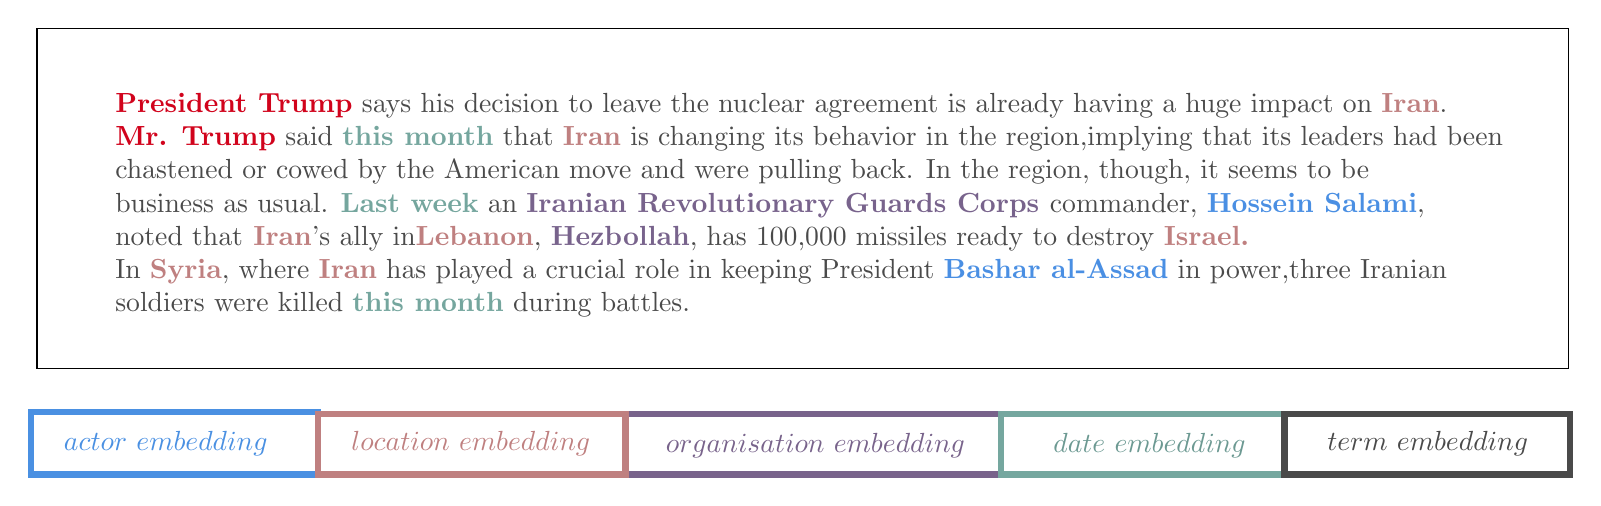
\begin{tikzpicture}[x=0.75pt,y=0.75pt,yscale=-1,xscale=1]
%uncomment if require: \path (0,300); %set diagram left start at 0, and has height of 300

\draw  [color={rgb, 255:red, 74; green, 144; blue, 226 }  ,draw opacity=1 ][line width=2.25]   (13, 207) rectangle (151.5, 237)   ;
\draw  [color={rgb, 255:red, 120; green, 99; blue, 139 }  ,draw opacity=1 ][line width=2.25]   (299.5, 208) rectangle (480.5, 237)   ;
\draw  [color={rgb, 255:red, 191; green, 128; blue, 128 }  ,draw opacity=1 ][line width=2.25]   (151.5, 208) rectangle (299.5, 237)   ;
\draw  [color={rgb, 255:red, 117; green, 167; blue, 159 }  ,draw opacity=1 ][line width=2.25]   (480.5, 208) rectangle (617, 237)   ;
\draw  [color={rgb, 255:red, 74; green, 74; blue, 74 }  ,draw opacity=1 ][line width=2.25]   (617, 208) rectangle (754.5, 237)   ;
\draw    (16, 22) rectangle (754, 186)   ;

\draw (78,222) node [color={rgb, 255:red, 74; green, 144; blue, 226 }  ,opacity=1 ]  {$actor\ embedding$};
\draw (225,222) node [color={rgb, 255:red, 191; green, 128; blue, 128 }  ,opacity=1 ]  {$location\ embedding$};
\draw (391,223) node [color={rgb, 255:red, 120; green, 99; blue, 139 }  ,opacity=1 ]  {$organisation\ embedding$};
\draw (552,223) node [color={rgb, 255:red, 108; green, 153; blue, 146 }  ,opacity=1 ]  {$date\ embedding$};
\draw (686,222) node [color={rgb, 255:red, 74; green, 74; blue, 74 }  ,opacity=1 ]  {$term\ embedding$};
\draw (388,130) node [scale=1,color={rgb, 255:red, 74; green, 74; blue, 74 }  ,opacity=1 ] [align=left] {\textcolor[rgb]{0.82,0.01,0.11}{\textbf{President Trump}} says his decision to leave the nuclear agreement is already having a huge impact on \textcolor[rgb]{0.75,0.5,0.5}{\textbf{Iran}}.\\\textcolor[rgb]{0.82,0.01,0.11}{\textbf{Mr. Trump}} said \textcolor[rgb]{0.46,0.65,0.62}{\textbf{this month}} that \textcolor[rgb]{0.75,0.5,0.5}{\textbf{Iran}} is changing its behavior in the region,implying that its leaders had been \\\textcolor[rgb]{0.29,0.29,0.29}{chastened or cowed by the American move and were pulling back. In the region, though, it seems to be}\\business as usual. \textcolor[rgb]{0.46,0.65,0.62}{\textbf{Last week}} an \textbf{\textcolor[rgb]{0.47,0.39,0.55}{Iranian Revolutionary Guards Corps} }commander, \textcolor[rgb]{0.29,0.56,0.89}{\textbf{Hossein Salami}}, \\noted that\textbf{ \textcolor[rgb]{0.75,0.5,0.5}{Iran}}’s ally in\textcolor[rgb]{0.75,0.5,0.5}{ \textbf{Lebanon}}, \textcolor[rgb]{0.47,0.39,0.55}{\textbf{Hezbollah}}, has 100,000 missiles ready to destroy \textbf{\textcolor[rgb]{0.75,0.5,0.5}{Israel.}} \\In \textcolor[rgb]{0.75,0.5,0.5}{\textbf{Syria}}, where \textcolor[rgb]{0.75,0.5,0.5}{\textbf{Iran}} has played a crucial role in keeping President \textcolor[rgb]{0.29,0.56,0.89}{\textbf{Bashar al-Assad}} in power,three Iranian \\soldiers were killed \textcolor[rgb]{0.46,0.65,0.62}{\textbf{this month}} during battles.\\\\\\};


\end{tikzpicture}

}
\caption{Faceted embedding of the entity \emph{``Donald Trump''} for a short paragraph. Each part of the embedding corresponds to the relation of the center word to that specific type. Each entity type is illustrated with matching color in text and embedding. }
\label{fig:faceted_emb}
\end{figure} 
\noindent
Some of the potential advantages and motivation for analysing each part separately are as follows: 
\begin{compactitem}
\item \emph{Interpretability of relations:} Since each part of the embedding vector encodes relations to one of the entity types, e.g., the actors part only encodes the actors in the context of a word. Through this separate components, the relations between two word or entities become more interpretable. Any similarity measure to compare two word vectors can be applied to each component separately. Thus, the similarity of the words can be broken down into their different attributes. If two entities are closer in location space and farther in actors space, it is possible that they are situated close locally, but are not related to the same people. \\

\item \emph{Change in meaning:} Exploring and visualizing different components of an embedding over time gives us insights into how that entity has evolved overtime, with respect to that component. When applied to a corpus with a temporal aspect, like news articles, faceted models can illustrate how a word changes its meaning in relation to different types. For example, \emph{``Donald Trump''} is mentioned frequently in location context with \emph{``Iran''} during the discussion for the nuclear deal, but some time after the abandonment of the deal the topic fades away and \emph{``Donald Trump''}  is mentioned more often with relation to other countries. This information can be extracted from the location subspace of the word embedding. Consequently, the values for the location part of the embedding will bring the word vector closer to any other entity that is also frequently mentioned with Iran deal during the nuclear discussions like \emph{``Khamenei''} (Iran's supreme leader). Even if \emph{``Khamenei''} is not directly mentioned with \emph{``Donald Trump''}, they are mentioned in the same context location-wise, and, therefore, are mapped to points close to each other in the location domain. If embeddings are reconstructed for a time span after the nuclear abandonment, the two mentioned entities should become less similar in location aspect. Although the same experiment can be done on normal embeddings, where all the words are treated equally, the distinguishable components give us additional insights as to what aspect has invoked the change.\\

\item \emph{Interpretability of evaluation tasks:} Separable parts also plays a role in interpretability of evaluation tasks. We experiment with using only a specific component in our evaluations in Chapter~\ref{chap:eval} to find out which type of entity surrounding a word is more influential for a certain task.\\

\item \emph{Flexible neighbourhood search:} With faceted models, the search for a similar word or entity becomes more flexible. Same as the embedding space, the search space can be divided into various types, where one can look for neighbours in a specific context. The type-specific information can be used in the search, where one can query for entities that are closer to a certain word in the temporal or location aspect. For example, \emph{``Washington''} as a political person should appear more often with the same actors and has a different actor dimension than \emph{``Washington DC''} as a location. The standard embedding treats all the word equally and therefore cannot reflect this type of similarity. Since the dimensions are independent and can be combined in an arbitrary way, a combination of different dimensions can tailor the search results further and create a type-specific search. 
\end{compactitem}
To achieve this type of embeddings, we define faceted embeddings as word embeddings, where each dimension represents the relation of the embedded word to a specific type of entities surrounding it. Which types are considered during training is arbitrary, but for the purpose of this work, we choose to contain actors, locations, organisations, dates, and terms, since these types are available by the LOAD model. An example of such an embedding vector ($w$) for a corpus containing types of actor (ACT), location (LOC), organisation (ORG), date (DAT) and term (TER) is shown below: \\
\mathleft
\begin{equation}
w=\left[ \underbrace { \begin{matrix}{ a }_{ 1,1 } ... { a }_{ 1,M } \end{matrix} } |\underbrace { \begin{matrix}{ a }_{ 1,M+1 } ... { a }_{ 1,2M } \end{matrix} } |\underbrace { \begin{matrix}{ a }_{ 1,2M+1 } ... { a }_{ 1,3M } \end{matrix} } |\underbrace { \begin{matrix}{ a }_{ 1,3M+1 } ... { a }_{ 1,4M } \end{matrix} } |\underbrace { \begin{matrix}{ a }_{ 14M+1 } ... { a }_{ 1,5M } \end{matrix} }  \right] 
\label{eq:concat_vec}
\end{equation}
$$ \quad  \mathrm{ACT} \quad  \qquad  \mathrm{LOC}\qquad \qquad \mathrm{ORG}\qquad \quad \qquad \mathrm{DAT}\qquad \quad  \qquad  \mathrm{TER}\qquad \qquad$$
\mathcenter
Provided that the most common dimension for word embeddings are between $100$ to $300$, to maintain the same order of dimension in faceted embeddings all the different parts have the same dimension but in a lower magnitude ($20$ to $50$). These small embeddings are concatenated to create the final embedding. Each part is independent of the rest and is usually trained separately.
With these independent components, the embeddings stand to be more interpretable. Although a model that divides the embedding space into entity types has not been studied, some work has been done to make the vector representations more interpretable. In the work of Frauqui et al. transformation of word vectors into sparse (and optionally binary) vectors is proposed~\brackettext{\cite{DBLP:journals/corr/FaruquiTYDS15}}. Each vector is projected into an over-complete binary vector, where each dimension represents a feature similar to ones used in traditional NLP systems but found automatically during training. However, since their dimensions are binary valued, there is no notion of the extent to which a word participates in a particular dimension. Later, a model based on rotating the word vectors was introduced in order to improve the interpretability.~\brackettext{\cite{DBLP:conf/emnlp/ParkBO17}}. Recently, a neural network-based approach to the problem was introduced by using sparse auto-encoders~\brackettext{\cite{DBLP:conf/aaai/SubramanianPJBH18}}. Although these works shine some light on the potential meaning of each dimension, they focus purely on terms. whereas, we generate embeddings that each part reflects the word related to entities of a certain type and takes more than terms into account. As explained in Chapter~\ref{chap:background}, the aim of the word embedding is to reduce the high dimensional space of text and embed words into a meaningful space, where words with similar meaning are mapped to points close to each other. In the case of faceted embedding, it is as if we are dividing the textual space into all possible entity types, where each subspace contains only entities of a specific type. To put it differently, the space of all words $V$ is represented as $V=A\bigcup  L\bigcup  O\bigcup  D\bigcup \overline {N} $, where $A$,$L$,$O$,$D$ are the sets of all actors, locations, organisations and, dates, respectively and $ T=\overline{N}$ denotes all the words which are not a named entity. The goal is then to map each word into all the subspaces, where words that co-occur with the same entities of a specific type are mapped closer together. Since all the subspaces are independent of each other (e.g., the space of all actors does not have any of the location entities inside it), each embedding learned on the different subspace is also independent. Hence, it is perfectly reasonable that two words are close in one subspace and far in another. \\
In the remainder of this chapter, we aim to introduce faceted models as a general framework for learning embeddings with known types and separable dimensions. To create such embeddings we propose three approaches, two of which are based on word embedding models and one use the graph embedding techniques: 
\begin{compactenum}
\item Modifying the cost function of the GloVe model to train a separate embedding for each entity type on an annotated corpus. Although the original GloVe uses the word co-occurrence matrix as input, we transform the model to use the adjacency matrix of a co-occurrence graph. 
\item Using a variation of the word2vec model, which supports an arbitrary definition of context for each word to train an embedding for each entity type. This model is also trained on a corpus annotated with named entities.
\item Extracting a co-occurrence graph from the annotated text and modifying the graph embedding model to generate embeddings based on neighbours of a specific type. 
\end{compactenum}
 %%%%%%%%%%%%%%%%%%%%%%%%%%%%%%%%%%%%%%%%%%%%%%%%%%%%%%%%%%%%
\section{Faceted GloVe}\label{sec:faceted_glove}
In the previous chapter, we indicated that the LOAD edge weight captures the corpus relations similar to the co-occurrence matrix and that meaning components can be extracted from them. In this chapter, we use this knowledge to create faceted embeddings from the weighted adjacency matrix of the LOAD graph. In the first part, the construction of a weighted adjacency matrix is illustrated followed by the model definition. We denote the faceted GloVe model by $f$GLV, where \emph{``f''} indicates the faceted model. The proposed model contains two type of cost functions, that are discussed separately in Section~\ref{sec:normal_cost} and~\ref{sec:unified_cost}. \\
The complete training task can be formulated in four steps: 
 \begin{enumerate}        
 \item Extraction of co-occurrence matrices for different types, explained in Section~\ref{sec:adj_matrix}. 
 \item For each type, a GloVe based embedding is learned using either a separate or unified cost function, discussed separately in Section~\ref{sec:normal_cost} and~\ref{sec:unified_cost}. 
 \item The context embedding is kept and the focal embedding is either disregarded to added with focal addition, discussed in Section~\ref{sec:faceted_embeddings}.
 \item The results of the third step are different embeddings for each type, which can be concatenated to generate the final faceted embedding. 
 \end{enumerate}
 %%%%%%%%%%%%%%%%%%%%%%%%%%%%%%%%%%%%%%%%%%%%%%%%%%%%%%%%%%%%
\subsection{Weighted adjacency matrix}\label{sec:adj_matrix}
To learn the embeddings, a weighted adjacency matrix for each type of entity and term is needed (ACT, LOC, TER, ORG, DAT). The matrices are constructed based on the weighted edge list of the co-occurrence graph, where the weights can be co-occurrence counts (identical to the GloVe model) or, any other distance measure defined by the graph. For example, the weighted adjacency matrix for actors contains the edges that have an actor as start nodes and any other type as the end node. Since in this thesis we use undirected co-occurrence graphs, the same edge exists in the opposite direction. For instance, an edge between an actor and a term is repeated twice and will be used once to create the actor matrix and once to create the term matrix. More formally, the matrices can be constructed as shown in Figure~\ref{fig:co-matrix}, where the entries of the matrices are the edge weights between two words.  
\begin{figure}
%\[\mathrm{ACT}=
%\begin{blockarray}{cccccccc}
% &\mathrm{TER}_1  & \color{myblue}{ \mathrm{ORG}_1 } &  \mathrm{TER}_2  & \mathrm{ACT}_1 & \mathrm{DAT}_1 & \mathrm{LOC}_1 & ... \\
%\begin{block}{c(ccccccc)}
%  \mathrm{ACT}_1 &m_{00} & \color{myblue}{ m_{01}}  &  m_{02} & m_{03} & m_{04} &m_{00}& ... \\
%  \mathrm{ACT}_2 & m_{10} & \color{myblue}{ m_{11} } &  m_{12} & m_{13} & m_{14} &m_{15}& ... \\
%  \mathrm{ACT}_3 & m_{20} &  \color{myblue}{m_{21} } &  m_{22} & m_{23} & m_{24} &m_{25}& ... \\
%  .. & ... &  \color{myblue}{...}  &  ... & ... & ... &...& ... \\
%\end{block}
%\end{blockarray}
% \]
%\[\mathrm{ORG}=
%\begin{blockarray}{cccccccc}
% &\mathrm{TER}_1  & \color{myblue}{ \mathrm{ORG}_1} &  \mathrm{TER}_2  & \mathrm{ACT}_1 & \mathrm{DAT}_1 & \mathrm{LOC}_1 & ... \\
%\begin{block}{c(ccccccc)}
%  \mathrm{ORG}_1 &m_{00} & \color{myblue}{ m_{01}}  &  m_{02} & m_{03} & m_{04} &m_{00}& ... \\
%  \mathrm{ORG}_2 & m_{10} & \color{myblue}{ m_{11} } &  m_{12} & m_{13} & m_{14} &m_{15}& ... \\
%  \mathrm{ORG} _3& m_{20} &  \color{myblue}{m_{21} } &  m_{22} & m_{23} & m_{24} &m_{25}& ... \\
%  .. & ... &  \color{myblue}{...}  &  ... & ... & ... &...& ... \\
%\end{block}
%\end{blockarray}
% \]
% \[\mathrm{DAT}=
%\begin{blockarray}{cccccccc}
% &TER1  & \color{myblue}{ \mathrm{ORG}_1} &  \mathrm{TER}_2  & \mathrm{ACT}_1 & \mathrm{DAT}_1 & \mathrm{LOC}_1 & ... \\
%\begin{block}{c(ccccccc)}
%  \mathrm{DAT}_1 &m_{00} & \color{myblue}{ m_{01}}  &  m_{02} & m_{03} & m_{04} &m_{00}& ... \\
%  \mathrm{DAT}_2 & m_{10} & \color{myblue}{ m_{11} } &  m_{12} & m_{13} & m_{14} &m_{15}& ... \\
%  \mathrm{DAT}_3 & m_{20} &  \color{myblue}{m_{21} } &  m_{22} & m_{23} & m_{24} &m_{25}& ... \\
%  .. & ... &  \color{myblue}{...}  &  ... & ... & ... &...& ... \\
%\end{block}
%\end{blockarray}
% \]
\centering 
\resizebox{0.97\textwidth}{0.26\textwidth}{      
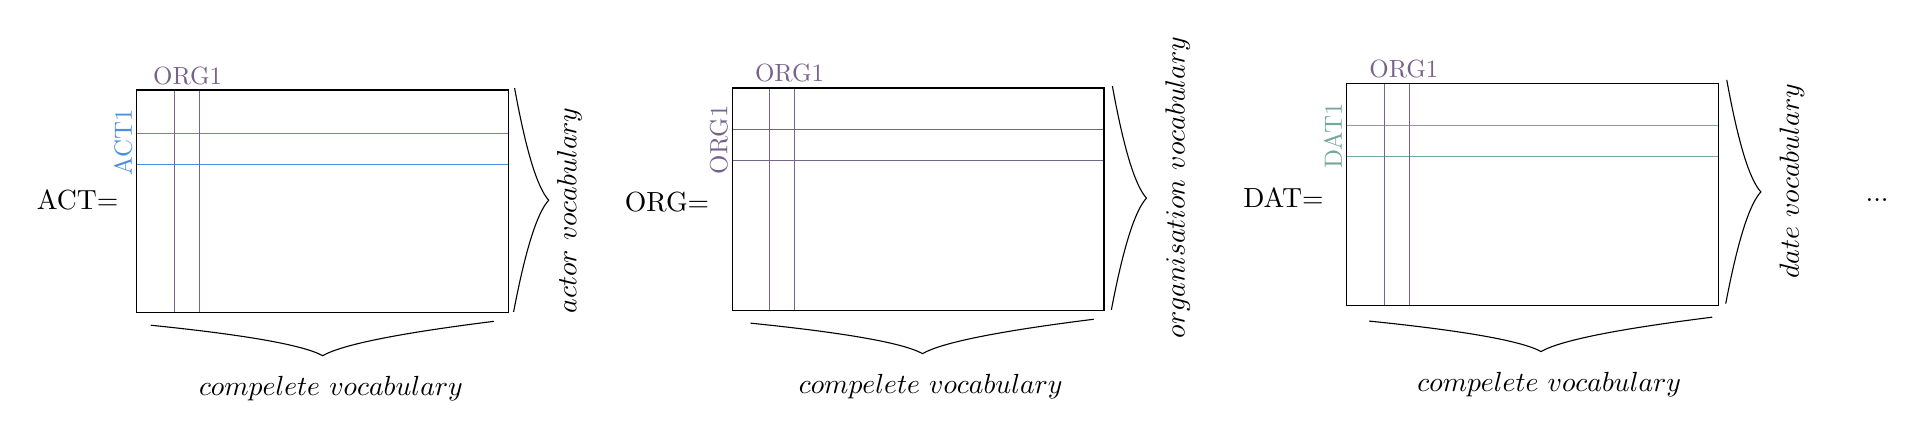
\begin{tikzpicture}[x=0.75pt,y=0.75pt,yscale=-1,xscale=1]
%uncomment if require: \path (0,370); %set diagram left start at 0, and has height of 370

%Shape: Rectangle [id:dp688565454623014] 
\draw  [color={rgb, 255:red, 74; green, 144; blue, 226 }  ,draw opacity=1 ] (55.5,122) -- (234.5,122) -- (234.5,137) -- (55.5,137) -- cycle ;
\draw   (227.55,212.43) .. controls (181.69,218.16) and (154.2,223.68) .. (145.07,228.99) .. controls (135.83,223.89) and (108.22,218.99) .. (62.24,214.31) ;
\draw   (237.54,100.09) .. controls (242.97,130.06) and (248.44,148.05) .. (253.97,154.07) .. controls (248.39,160.03) and (242.75,177.97) .. (237.05,207.89) ;
%Shape: Rectangle [id:dp37213328100124254] 
\draw  [color={rgb, 255:red, 120; green, 99; blue, 139 }  ,draw opacity=1 ] (73.5,101) -- (85.5,101) -- (85.5,208) -- (73.5,208) -- cycle ;
%Shape: Rectangle [id:dp4064945973146499] 
\draw  [color={rgb, 255:red, 0; green, 0; blue, 0 }  ,draw opacity=1 ] (55.5,101) -- (234.5,101) -- (234.5,208) -- (55.5,208) -- cycle ;
%Shape: Rectangle [id:dp5929123930060234] 
\draw  [color={rgb, 255:red, 120; green, 99; blue, 139 }  ,draw opacity=1 ] (342.5,120) -- (521.5,120) -- (521.5,135) -- (342.5,135) -- cycle ;
%Shape: Rectangle [id:dp5111732488988676] 
\draw  [color={rgb, 255:red, 120; green, 99; blue, 139 }  ,draw opacity=1 ] (360.5,100) -- (372.5,100) -- (372.5,207) -- (360.5,207) -- cycle ;
%Shape: Rectangle [id:dp03627212507715449] 
\draw  [color={rgb, 255:red, 0; green, 0; blue, 0 }  ,draw opacity=1 ] (342.5,100) -- (521.5,100) -- (521.5,207) -- (342.5,207) -- cycle ;
%Shape: Rectangle [id:dp8482224250536965] 
\draw  [color={rgb, 255:red, 117; green, 167; blue, 159 }  ,draw opacity=1 ] (638.5,118) -- (817.5,118) -- (817.5,133) -- (638.5,133) -- cycle ;
%Shape: Rectangle [id:dp9261416839296721] 
\draw  [color={rgb, 255:red, 120; green, 99; blue, 139 }  ,draw opacity=1 ] (656.5,98) -- (668.5,98) -- (668.5,205) -- (656.5,205) -- cycle ;
%Shape: Rectangle [id:dp8074449392219452] 
\draw  [color={rgb, 255:red, 0; green, 0; blue, 0 }  ,draw opacity=1 ] (638.5,98) -- (817.5,98) -- (817.5,205) -- (638.5,205) -- cycle ;
\draw   (516.55,211.43) .. controls (470.69,217.16) and (443.2,222.68) .. (434.07,227.99) .. controls (424.83,222.89) and (397.22,217.99) .. (351.24,213.31) ;
\draw   (814.55,210.43) .. controls (768.69,216.16) and (741.2,221.68) .. (732.07,226.99) .. controls (722.83,221.89) and (695.22,216.99) .. (649.24,212.31) ;
\draw   (525.54,99.09) .. controls (530.97,129.06) and (536.44,147.05) .. (541.97,153.07) .. controls (536.39,159.03) and (530.75,176.97) .. (525.05,206.89) ;
\draw   (821.54,96.09) .. controls (826.97,126.06) and (832.44,144.05) .. (837.97,150.07) .. controls (832.39,156.03) and (826.75,173.97) .. (821.05,203.89) ;

% Text Node
\draw (80,94) node [scale=0.9,color={rgb, 255:red, 120; green, 99; blue, 139 }  ,opacity=1 ] [align=left] {ORG1};
% Text Node
\draw (149,245) node   {$compelete\ vocabulary$};
% Text Node
\draw (264,159) node [rotate=-270]  {$actor\ vocabulary$};
% Text Node
\draw (49,126) node [scale=0.9,color={rgb, 255:red, 74; green, 144; blue, 226 }  ,opacity=1 ,rotate=-270] [align=left] {ACT1};
% Text Node
\draw (370,93) node [scale=0.9,color={rgb, 255:red, 120; green, 99; blue, 139 }  ,opacity=1 ] [align=left] {ORG1};
% Text Node
\draw (557,148) node [rotate=-270]  {$organisation\ vocabulary$};
% Text Node
\draw (336,125) node [scale=0.9,color={rgb, 255:red, 120; green, 99; blue, 139 }  ,opacity=1 ,rotate=-270] [align=left] {ORG1};
% Text Node
\draw (666,91) node [scale=0.9,color={rgb, 255:red, 120; green, 99; blue, 139 }  ,opacity=1 ] [align=left] {ORG1};
% Text Node
\draw (853,145) node [rotate=-270]  {$date\ vocabulary$};
% Text Node
\draw (632,123) node [scale=0.9,color={rgb, 255:red, 117; green, 167; blue, 159 }  ,opacity=1 ,rotate=-270] [align=left] {DAT1};
% Text Node
\draw (894,154) node   {$...$};
% Text Node
\draw (27,154) node  [align=left] {ACT=};
% Text Node
\draw (311,155) node  [align=left] {ORG=};
% Text Node
\draw (608,153) node  [align=left] {DAT=};
% Text Node
\draw (438,244) node   {$compelete\ vocabulary$};
% Text Node
\draw (736,243) node   {$compelete\ vocabulary$};


\end{tikzpicture}

}
 \caption{Faceted weighted adjacency matrix. For each type of entity a weighted adjacency matrix is created, which contains all the entities of that type on the rows and all the words in the vocabulary in the columns.}
 \label{fig:co-matrix}
\end{figure}
The columns marked in blue in matrices $\mathrm{ACT}\in R^{|V_{\mathrm{ACT}}|\times |V|}$ , $ORG\in R^{|V_{\mathrm{ORG}}|\times |V|}$  and $\mathrm{DAT}\in R^{|V_{\mathrm{DAT}}|\times |V|}$ will be used to learn the actor, organisation and date part of the ORG$_1$embedding respectively. The complete vocabulary is divided into words belonging into each entity type. As a result, if $V$ is the complete vocabulary and $V_{\mathrm{ACT}}$,$V_{\mathrm{LOC}}$ $V_{\mathrm{ORG}}$, $V_{\mathrm{DAT}}$, and $V_{\mathrm{TER}}$ are the set of all actors, location, organization, dates, and terms in the graph, we will have $V=V_{\mathrm{ACT}}+V_{\mathrm{LOC}}+V_{\mathrm{ORG}}+V_{\mathrm{DAT}}+V_{\mathrm{TER}}$. The model will learn an embedding for all entities in the row and all entities in the column of the matrix. In case of a symmetric co-occurrence matrix the model learns the same embedding twice. Nevertheless, in our case the matrices are not symmetric and that leads to a definition of a new cost function, where this asymmetry is taken into account.
 %%%%%%%%%%%%%%%%%%%%%%%%%%%%%%%%%%%%%%%%%%%%%%%%%%%%%%%%%%%%
\subsection{Cost function of faceted embeddings}
\label{sec:faceted_embeddings}
For each different adjacency matrix, different embeddings need to be learned. To train all embeddings, two methods are proposed. First, training a network for each type separately and concatenating the outputs to generate the faceted embeddings. Second, train all the embeddings at once in a single network with a unified cost function. We refer to separate and unified cost function as $f$GLV$_{sep}$ and $f$GLV$_{uni}$, respectively.  the second method, despite the compactness, is slower than optimising separate cost functions. It is worth noting that the switching between the training method has no effect on the quality of embeddings, only the training time. For the sake of completeness however, we present both methods. Below we consider some alteration to the cost function of original GloVe that are considered to make faceted embedding possible and also to achieve better results. 
\begin{compactitem}
\item \emph{Asymmetry of context and focal embeddings:} Similar to GloVe embeddings for both context and focal are learned, but the focal embedding can no longer be naively summed up with the context. Instead, the focal embeddings can either be disregarded completely or added in a new way. For this purpose, we propose selectional addition, where the focal embedding of a certain type is only added to the corresponding embedding in the context. As an example, take the adjacency matrices in Section~\ref{sec:adj_matrix} as our input, then for the matrix ACT,  focal embedding will learn to encode each row, while the context will encode the columns. The rows of the matrix will represent embeddings of all the actors with respect to the whole vocabulary. We are interested in column embeddings that encode the actor part for all the words in our vocabulary, which is the purpose of this model. Focal embedding also contains information about the whole vocabulary, but only for the focal words (actors), adding back this information in terms of selectional addition is beneficial to the model. The selectional addition adds the focal embedding of a type only to the respective entities of that type in the context matrix. The rest of embeddings remain intact, because a corresponding embedding column for them in the focal matrix does not exist. A visualization of the focal addition for type actor can be seen in Figure~\ref{fig:focal_addition}.\\

\item \emph{Final concatenation:} The output of the model is an embedding for each type. These vectors can later be combined to generate the complete faceted embedding. As the embeddings are independent, the combination can be arbitrary with only the desired dimensions kept. \\

\item \emph{Weighting function:} The weighting function ($f(X_{ij})$) is the weighting function for GloVe. The model is valid with or without the use of a weighting function, but since the weights of a co-occurrence graph are highly unbalanced, without a weighting function, very large weights will overpower the smaller ones and reduce performance. Therefore cutting off the weights at a certain threshold can to some extent balance out this effect. The hyperparameters of the weighting function should be tuned based on the dataset.\\

\item \emph{Normalization:} Some variations to the model were experimented with, but because of extremely poor results were disregard. One of such approaches is edge weight normalization. In an attempt to boost performance, weights of the graph were normalized using logarithmic normalization. With normalization, we reduce the range of values, in which the weights fluctuate. Moreover, the gradient descent algorithm can converge more smoothly to the functions minimum. Unfortunately, adding the normalization for the GloVe model made the problem ill-conditioned and the algorithm could not converge to a solution and, therefore, is dismissed. The reason for this could be that the normalization $log$ might result in negative values. In the cost function, a second $log$ is applied to the inputs, and the $log$ of a negative number is undefined, resulting in undefined gradient updates and untrainable weights. Other than log normalization, a linear transformation like \emph{min max normalization} was also experimented. Min-max normalization forces all the weights to be between $0$ and $1$ and is calculated with Equation~\ref{eq:minmaxNom}, where $e=(e_1,...,e_n)$ is the set of input weights and $z_i$ is the $i$th normalized data. Unfortunately, adding this form of normalization does not improve the results and is also removed from the model.
\begin{equation}
z_{ i }=\frac { e_{ i }-min(e) }{ max(e)-min(e) } 
\label{eq:minmaxNom}
\end{equation}

\item \emph{Adding $1$ to the logarithm:} The cost function applies a logarithm to the weights. For an edge weight of $1$ the $log(1)=0$. Therefore, we tested the model with the addition of $1$ to the $log$ of weights, to adjust for this effect. With this change, the cost function is changed to Equation~\ref{eq:log_plus}. Although in some cases this change improved the model performance, in other cases it generated poor results. More details about how this change affects the model is discussed in Section~\ref{sec:setup}. 
\begin{equation}
J_e=\sum _{ j=1 }^{ |V| }{}\sum _{ i=1 }^{ |V_f| }{ f({ X }_{ ij } } )(w_{ i }^{ T }\tilde{  w_{ j } } +b_{ i }+\tilde{  b_{ j } } -(log{ X }_{ ij }+1))^2
\label{eq:log_plus}
\end{equation}
\end{compactitem}
All the discussed alterations to the original cost function of GloVe can be applied to both unified and separate cost function. In the following, we discus the two cost functions for faceted GloVe and explain their difference. 
 %%%%%%%%%%%%%%%%%%%%%%%%%%%%%%%%%%%%%%%%%%%%%%%%%%%%%%%%%%%%
\subsubsection{Separate cost functions}
\label{sec:normal_cost}

The general cost function for a single network is the one used for the GloVe model with minor modifications.
As noted in the previous section, context and focal embeddings are no longer symmetric like the GloVe model, since the size of context vocabulary is different from the focal. 
By limiting the focal words to a certain type we try to infer the impact of that type on all the words and generate type-specific embeddings. Accordingly, the context embedding in each case reflects these type-specific properties for all words. The biases can no longer be symmetric as well. Therefore, the GloVe cost function can be re-written to Equation~\ref{eq:sep_cost}, where $V_f$ is the size of the focal vocabulary.
\begin{equation}
J_e=\sum _{ j=1 }^{ |V| }{}\sum _{ i=1 }^{ |V_f| }{ f({ X }_{ ij } } )(w_{ i }^{ \top }\tilde{  w_{ j } } +b_{ i }+\tilde{  b_{ j } } -log{ X }_{ ij })^2
\label{eq:sep_cost}
\end{equation}
The cost function has to be minimized separately for each entity type. Thus, the training will contain a separate training phases for each type and a final concatenation. 
 %%%%%%%%%%%%%%%%%%%%%%%%%%%%%%%%%%%%%%%%%%%%%%%%%%%%%%%%%%%%
\subsubsection{Unified cost function  }
\label{sec:unified_cost}
The unified cost function is simply the summation of all the separate cost functions in the previous section, where $K$ is the set of all possible types, shown in Equation~\ref{eq:unified_cost}.
\begin{equation}
J=\sum _{ k=1 }^{ |K| }{J_k}=\sum _{ k=1 }^{ |K| }{}\sum _{ j=1 }^{ |V| }{}\sum _{ i=1 }^{ |V_f| }{ f({ X }_{ ij } } )(w_{ i }^{ \top }\tilde{  w_{ j } } +b_{ i }+\tilde{  b_{ j } } -log{ X }_{ ij })^2
\label{eq:unified_cost}
\end{equation}
As a result, all embeddings can be generated with a single network. For a better understanding of the differences between the methods a visual comparison is shown in Figures~\ref{fig:separate_cost} and~\ref{fig:unified_cost} for a loss on a single input. Each input is an edge with its corresponding weight, if the input has the starting node of type actor, the rest of the layers related to other types of embeddings will be frozen during training and only the weights for the actor network will be updated through backpropagation. Hence, it is as if all the networks were trained separately.  \\
In Figure~\ref{fig:separate_cost}, two networks are shown as an example. A single edge refers to two embeddings, one for the focal (start node) and one for the context (end node). Each network is trained separately and a final embedding for a single context word is the concatenation of all learned embeddings. \\
In contrast, in Figure~\ref{fig:unified_cost}, one network with five times more parameters is trained, where each input edge only affects the weight of the network associated with the focal word (start node). Therefore, an edge between an actor and term does not affect the location related embedding. Since the edges are undirected, the edge in the opposite direction will be fed as an input to the term network and hence no information is lost. All other aspects discussed for faceted embeddings with a separate cost function (focal addition, normalization and \dots) also applies to the unified cost function.
\begin{figure}
{\small 
\tikzset{every picture/.style={line width=0.75pt}} %set default line width to 0.75pt        
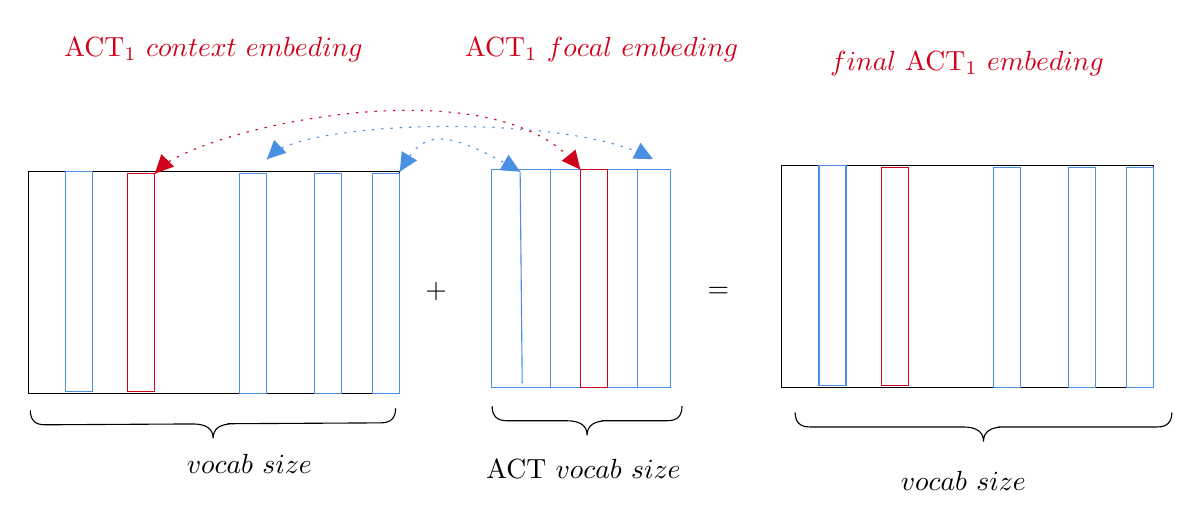
\begin{tikzpicture}[x=0.75pt,y=0.75pt,yscale=-1,xscale=1]
%uncomment if require: \path (0,370); %set diagram left start at 0, and has height of 370

\draw    (16.5, 126) rectangle (195.5, 233)   ;
\draw  [color={rgb, 255:red, 74; green, 144; blue, 226 }  ,draw opacity=1 ]  (239.75, 125) rectangle (326, 230)   ;
\draw   (17.5,241) .. controls (17.53,245.67) and (19.87,247.99) .. (24.54,247.96) -- (95.54,247.55) .. controls (102.21,247.51) and (105.55,249.82) .. (105.58,254.49) .. controls (105.55,249.82) and (108.87,247.47) .. (115.54,247.44)(112.54,247.45) -- (186.54,247.03) .. controls (191.21,247) and (193.53,244.66) .. (193.5,239.99) ;
\draw   (240,239) .. controls (240,243.67) and (242.33,246) .. (247,246) -- (275.75,246) .. controls (282.42,246) and (285.75,248.33) .. (285.75,253) .. controls (285.75,248.33) and (289.08,246) .. (295.75,246)(292.75,246) -- (324.5,246) .. controls (329.17,246) and (331.5,243.67) .. (331.5,239) ;
\draw  [color={rgb, 255:red, 208; green, 2; blue, 27 }  ,draw opacity=1 ]  (64.5, 127) rectangle (77.5, 232)   ;
\draw  [color={rgb, 255:red, 208; green, 2; blue, 27 }  ,draw opacity=1 ]  (282.5, 125) rectangle (295.5, 230)   ;
\draw   (386,242) .. controls (386,246.67) and (388.33,249) .. (393,249) -- (466.75,249) .. controls (473.42,249) and (476.75,251.33) .. (476.75,256) .. controls (476.75,251.33) and (480.08,249) .. (486.75,249)(483.75,249) -- (560.5,249) .. controls (565.17,249) and (567.5,246.67) .. (567.5,242) ;
\draw    (268, 125) rectangle (268, 230)   ;
\draw    (310.25, 125) rectangle (310.25, 229)   ;
\draw [color={rgb, 255:red, 74; green, 144; blue, 226 }  ,draw opacity=1 ]   (253.5,126) -- (254.5,228) ;


\draw [color={rgb, 255:red, 74; green, 144; blue, 226 }  ,draw opacity=1 ]   (268,125) -- (268,230) ;


\draw [color={rgb, 255:red, 74; green, 144; blue, 226 }  ,draw opacity=1 ]   (310.25,125) -- (310.25,230) ;


\draw [color={rgb, 255:red, 74; green, 144; blue, 226 }  ,draw opacity=1 ]   (326,125) -- (326,230) ;


\draw  [color={rgb, 255:red, 74; green, 144; blue, 226 }  ,draw opacity=1 ]  (118.5, 127) rectangle (131.5, 233)   ;
\draw  [color={rgb, 255:red, 74; green, 144; blue, 226 }  ,draw opacity=1 ]  (182.5, 127) rectangle (195.5, 233)   ;
\draw [color={rgb, 255:red, 74; green, 144; blue, 226 }  ,draw opacity=1 ] [dash pattern={on 0.84pt off 2.51pt}]  (195.5,126) .. controls (206.5,107) and (213.5,103) .. (253.5,126) ;
\draw [shift={(253.5,126)}, rotate = 209.57999999999998] [fill={rgb, 255:red, 74; green, 144; blue, 226 }  ,fill opacity=1 ] [draw opacity=0] (8.93,-4.29) -- (0,0) -- (8.93,4.29) -- (8.93,-4.29)    ;
\draw [shift={(195.5,126)}, rotate = 301.28] [fill={rgb, 255:red, 74; green, 144; blue, 226 }  ,fill opacity=1 ] [draw opacity=0] (8.93,-4.29) -- (0,0) -- (8.93,4.29) -- (8.93,-4.29)    ;
\draw [color={rgb, 255:red, 74; green, 144; blue, 226 }  ,draw opacity=1 ] [dash pattern={on 0.84pt off 2.51pt}]  (131.5,120) .. controls (142.5,101) and (277.5,97) .. (317.5,120) ;
\draw [shift={(317.5,120)}, rotate = 207.42000000000002] [fill={rgb, 255:red, 74; green, 144; blue, 226 }  ,fill opacity=1 ] [draw opacity=0] (8.93,-4.29) -- (0,0) -- (8.93,4.29) -- (8.93,-4.29)    ;
\draw [shift={(131.5,120)}, rotate = 316.16] [fill={rgb, 255:red, 74; green, 144; blue, 226 }  ,fill opacity=1 ] [draw opacity=0] (8.93,-4.29) -- (0,0) -- (8.93,4.29) -- (8.93,-4.29)    ;
\draw [color={rgb, 255:red, 208; green, 2; blue, 27 }  ,draw opacity=1 ] [dash pattern={on 0.84pt off 2.51pt}]  (77.5,127) .. controls (88.5,108) and (241.5,70) .. (282.5,125) ;
\draw [shift={(282.5,125)}, rotate = 230.89] [fill={rgb, 255:red, 208; green, 2; blue, 27 }  ,fill opacity=1 ] [draw opacity=0] (8.93,-4.29) -- (0,0) -- (8.93,4.29) -- (8.93,-4.29)    ;
\draw [shift={(77.5,127)}, rotate = 313.85] [fill={rgb, 255:red, 208; green, 2; blue, 27 }  ,fill opacity=1 ] [draw opacity=0] (8.93,-4.29) -- (0,0) -- (8.93,4.29) -- (8.93,-4.29)    ;
\draw  [color={rgb, 255:red, 74; green, 144; blue, 226 }  ,draw opacity=1 ]  (154.5, 127) rectangle (167.5, 233)   ;
\draw  [color={rgb, 255:red, 74; green, 144; blue, 226 }  ,draw opacity=1 ]  (34.5, 126) rectangle (47.5, 232)   ;
\draw    (379.5, 123) rectangle (558.5, 230)   ;
\draw  [color={rgb, 255:red, 208; green, 2; blue, 27 }  ,draw opacity=1 ]  (427.5, 124) rectangle (440.5, 229)   ;
\draw  [color={rgb, 255:red, 74; green, 144; blue, 226 }  ,draw opacity=1 ]  (481.5, 124) rectangle (494.5, 230)   ;
\draw  [color={rgb, 255:red, 74; green, 144; blue, 226 }  ,draw opacity=1 ]  (545.5, 124) rectangle (558.5, 230)   ;
\draw  [color={rgb, 255:red, 74; green, 144; blue, 226 }  ,draw opacity=1 ]  (517.5, 124) rectangle (530.5, 230)   ;
\draw  [color={rgb, 255:red, 74; green, 144; blue, 226 }  ,draw opacity=1 ]  (397.5, 123) rectangle (410.5, 229)   ;

\draw (124,186) node   {$\stackrel{}{}$};
\draw (213,184) node   {$+$};
\draw (349,184) node   {$=$};
\draw (123,267) node   {$vocab\ size$};
\draw (284,269) node   {$\mathrm{ACT}\ vocab\ size$};
\draw (108,67) node [color={rgb, 255:red, 208; green, 2; blue, 27 }  ,opacity=1 ]  {$\mathrm{ACT}_1\ context\ embeding\ $};
\draw (295,67) node [color={rgb, 255:red, 208; green, 2; blue, 27 }  ,opacity=1 ]  {$\mathrm{ACT}_1\ focal\ embeding\ $};
\draw (471,74) node [color={rgb, 255:red, 208; green, 2; blue, 27 }  ,opacity=1 ]  {$final\ \mathrm{ACT}_1\ embeding\ $};
\draw (467,275) node [color={rgb, 255:red, 0; green, 0; blue, 0 }  ,opacity=1 ]  {$vocab\ size$};
\draw (487,183) node   {$\stackrel{}{}$};


\end{tikzpicture}



}
\caption{Selectional addition of focal and context embedding in case of the actor embeddings. ACT$_1$ is shown as an example, where embeddings in focal and context matrices are combined to make the final embedding.} \label{fig:focal_addition}
\end{figure}

\begin{figure}
{\small 
\tikzset{every picture/.style={line width=0.75pt}} %set default line width to 0.75pt        

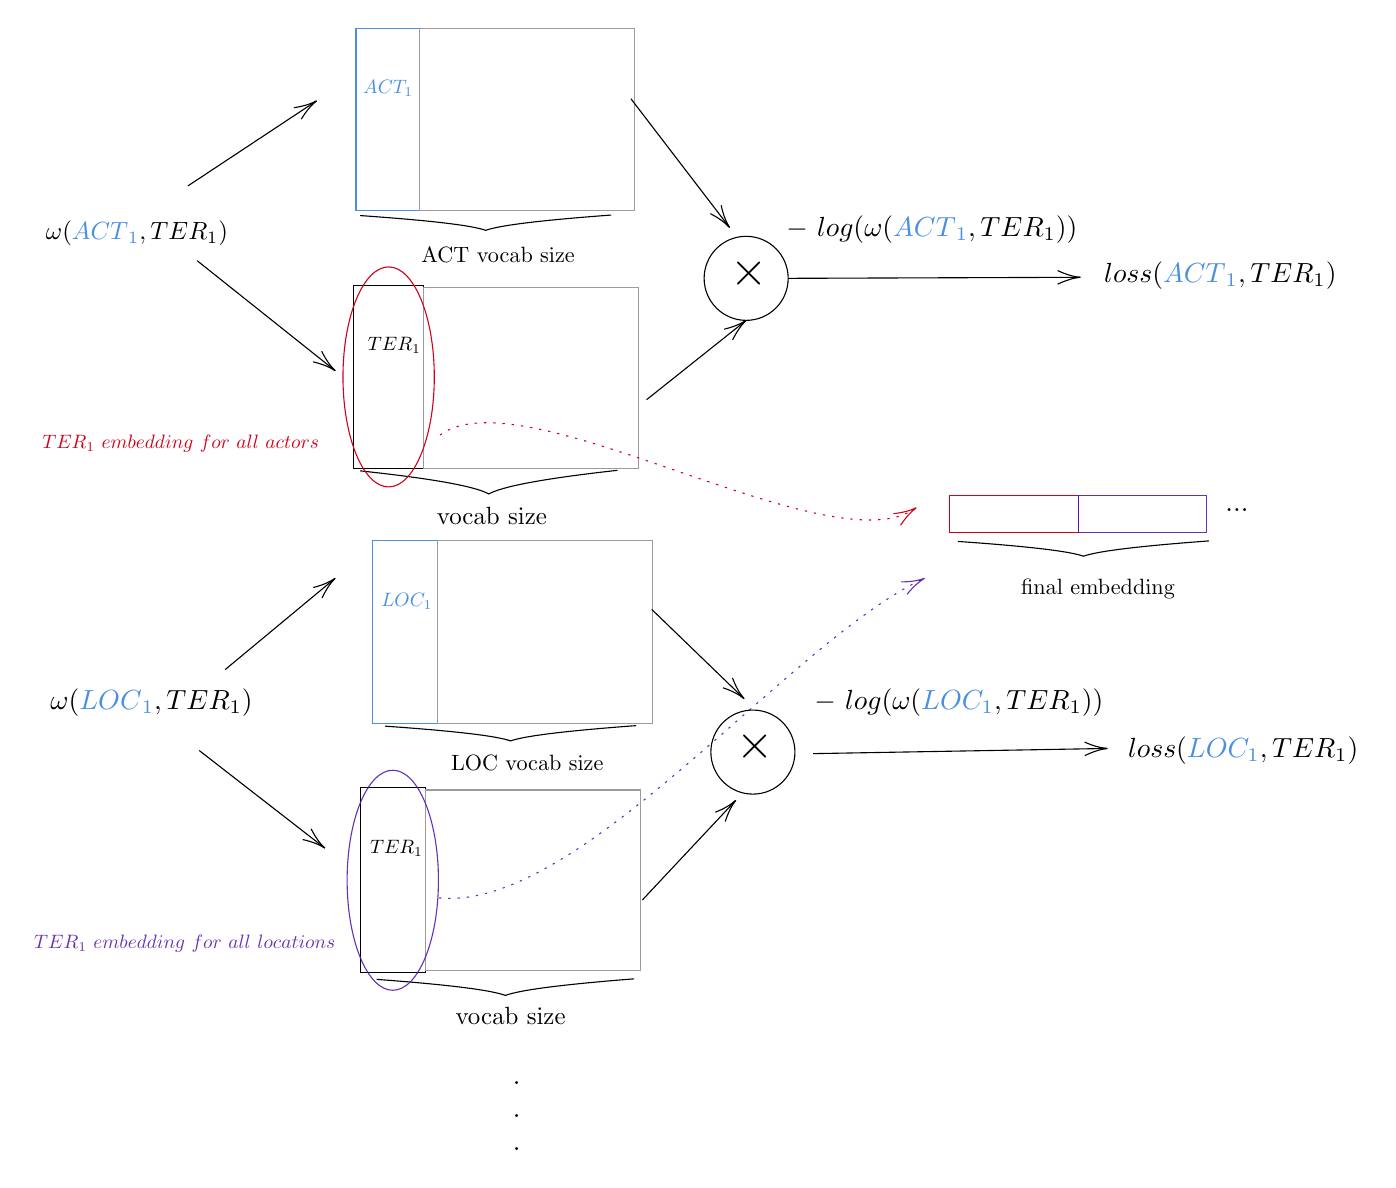
\begin{tikzpicture}[x=0.75pt,y=0.75pt,yscale=-1,xscale=1]
%uncomment if require: \path (0,573); %set diagram left start at 0, and has height of 573

\draw    (373.75,127.5) -- (514.5,127) ;
\draw [shift={(514.5,127)}, rotate = 539.8] [color={rgb, 255:red, 0; green, 0; blue, 0 }  ]   (0,0) .. controls (3.31,-0.3) and (6.95,-1.4) .. (10.93,-3.29)(0,0) .. controls (3.31,0.3) and (6.95,1.4) .. (10.93,3.29)   ;

\draw    (84.5,83) -- (146.5,42) ;
\draw [shift={(146.5,42)}, rotate = 506.52] [color={rgb, 255:red, 0; green, 0; blue, 0 }  ]   (0,0) .. controls (3.31,-0.3) and (6.95,-1.4) .. (10.93,-3.29)(0,0) .. controls (3.31,0.3) and (6.95,1.4) .. (10.93,3.29)   ;

\draw  [color={rgb, 255:red, 74; green, 144; blue, 226 }  ,draw opacity=1 ]  (165.5, 7) rectangle (196, 95)   ;
\draw    (164.5, 131) rectangle (198, 219)   ;
\draw  [color={rgb, 255:red, 155; green, 155; blue, 155 }  ,draw opacity=1 ]  (196, 7) rectangle (299.5, 95)   ;
\draw  [color={rgb, 255:red, 155; green, 155; blue, 155 }  ,draw opacity=1 ]  (198, 132) rectangle (301.5, 219)   ;
\draw [rotate around= { 89.88: (229.51, 225.75)
    }]  (223.89,163.75) .. controls (227.64,198.19) and (231.38,218.86) .. (235.13,225.75) .. controls (231.38,232.64) and (227.64,253.31) .. (223.89,287.75) ;
\draw [rotate around= { 89.88: (228.01, 100.75)
    }]  (224.39,40.25) .. controls (226.8,73.86) and (229.22,94.03) .. (231.63,100.75) .. controls (229.22,107.47) and (226.8,127.64) .. (224.39,161.25) ;
\draw    (353.5, 127.5) circle [x radius= 20.25, y radius= 20.25]  ;
\draw    (305.5,186) -- (353.5,147.75) ;
\draw [shift={(353.5,147.75)}, rotate = 501.45] [color={rgb, 255:red, 0; green, 0; blue, 0 }  ]   (0,0) .. controls (3.31,-0.3) and (6.95,-1.4) .. (10.93,-3.29)(0,0) .. controls (3.31,0.3) and (6.95,1.4) .. (10.93,3.29)   ;

\draw    (298,41) -- (345.5,103) ;
\draw [shift={(345.5,103)}, rotate = 232.54] [color={rgb, 255:red, 0; green, 0; blue, 0 }  ]   (0,0) .. controls (3.31,-0.3) and (6.95,-1.4) .. (10.93,-3.29)(0,0) .. controls (3.31,0.3) and (6.95,1.4) .. (10.93,3.29)   ;

\draw    (90,355) -- (150.5,402) ;
\draw [shift={(150.5,402)}, rotate = 217.84] [color={rgb, 255:red, 0; green, 0; blue, 0 }  ]   (0,0) .. controls (3.31,-0.3) and (6.95,-1.4) .. (10.93,-3.29)(0,0) .. controls (3.31,0.3) and (6.95,1.4) .. (10.93,3.29)   ;

\draw    (102.5,316) -- (155.5,272) ;
\draw [shift={(155.5,272)}, rotate = 500.3] [color={rgb, 255:red, 0; green, 0; blue, 0 }  ]   (0,0) .. controls (3.31,-0.3) and (6.95,-1.4) .. (10.93,-3.29)(0,0) .. controls (3.31,0.3) and (6.95,1.4) .. (10.93,3.29)   ;

\draw  [color={rgb, 255:red, 74; green, 144; blue, 226 }  ,draw opacity=1 ]  (173.5, 254) rectangle (205, 342)   ;
\draw    (167.5, 373) rectangle (199, 462)   ;
\draw  [color={rgb, 255:red, 155; green, 155; blue, 155 }  ,draw opacity=1 ]  (205, 254) rectangle (308.5, 342)   ;
\draw  [color={rgb, 255:red, 155; green, 155; blue, 155 }  ,draw opacity=1 ]  (199, 374) rectangle (302.5, 461)   ;
\draw [rotate around= { 89.88: (237.51, 469.07)
    }]  (233.57,407.07) .. controls (236.2,441.51) and (238.82,462.18) .. (241.44,469.07) .. controls (238.82,475.95) and (236.2,496.62) .. (233.57,531.07) ;
\draw    (356.75, 355.75) circle [x radius= 20.25, y radius= 20.25]  ;
\draw    (303.5,427) -- (348.5,379) ;
\draw [shift={(348.5,379)}, rotate = 493.15] [color={rgb, 255:red, 0; green, 0; blue, 0 }  ]   (0,0) .. controls (3.31,-0.3) and (6.95,-1.4) .. (10.93,-3.29)(0,0) .. controls (3.31,0.3) and (6.95,1.4) .. (10.93,3.29)   ;

\draw    (308,287) -- (352.5,330) ;
\draw [shift={(352.5,330)}, rotate = 224.02] [color={rgb, 255:red, 0; green, 0; blue, 0 }  ]   (0,0) .. controls (3.31,-0.3) and (6.95,-1.4) .. (10.93,-3.29)(0,0) .. controls (3.31,0.3) and (6.95,1.4) .. (10.93,3.29)   ;

\draw [rotate around= { 89.88: (240.01, 346.75)
    }]  (236.39,286.25) .. controls (238.8,319.86) and (241.22,340.03) .. (243.63,346.75) .. controls (241.22,353.47) and (238.8,373.64) .. (236.39,407.25) ;
\draw  [color={rgb, 255:red, 208; green, 2; blue, 27 }  ,draw opacity=1 ]  (181.25, 175) circle [x radius= 22, y radius= 53]  ;
\draw  [color={rgb, 255:red, 82; green, 21; blue, 168 }  ,draw opacity=0.88 ]  (183.25, 417.5) circle [x radius= 22, y radius= 53]  ;
\draw [color={rgb, 255:red, 208; green, 2; blue, 27 }  ,draw opacity=1 ] [dash pattern={on 0.84pt off 2.51pt}]  (206,203) .. controls (246,173) and (395.5,268) .. (435.5,238) ;
\draw [shift={(435.5,238)}, rotate = 508.65] [color={rgb, 255:red, 208; green, 2; blue, 27 }  ,draw opacity=1 ]   (0,0) .. controls (3.31,-0.3) and (6.95,-1.4) .. (10.93,-3.29)(0,0) .. controls (3.31,0.3) and (6.95,1.4) .. (10.93,3.29)   ;

\draw [color={rgb, 255:red, 82; green, 21; blue, 168 }  ,draw opacity=0.88 ] [dash pattern={on 0.84pt off 2.51pt}]  (205.5,426) .. controls (273.5,433) and (375.5,301) .. (439.5,272) ;
\draw [shift={(439.5,272)}, rotate = 514.4] [color={rgb, 255:red, 82; green, 21; blue, 168 }  ,draw opacity=0.88 ]   (0,0) .. controls (3.31,-0.3) and (6.95,-1.4) .. (10.93,-3.29)(0,0) .. controls (3.31,0.3) and (6.95,1.4) .. (10.93,3.29)   ;

\draw  [color={rgb, 255:red, 208; green, 2; blue, 27 }  ,draw opacity=1 ]  (451.5, 232) rectangle (513.5, 250)   ;
\draw  [color={rgb, 255:red, 82; green, 21; blue, 168 }  ,draw opacity=0.88 ]  (513.5, 232) rectangle (575.5, 250)   ;
\draw    (89,119) -- (155.5,172) ;
\draw [shift={(155.5,172)}, rotate = 218.55] [color={rgb, 255:red, 0; green, 0; blue, 0 }  ]   (0,0) .. controls (3.31,-0.3) and (6.95,-1.4) .. (10.93,-3.29)(0,0) .. controls (3.31,0.3) and (6.95,1.4) .. (10.93,3.29)   ;

\draw    (385.75,356.5) -- (527.5,354) ;
\draw [shift={(527.5,354)}, rotate = 538.99] [color={rgb, 255:red, 0; green, 0; blue, 0 }  ]   (0,0) .. controls (3.31,-0.3) and (6.95,-1.4) .. (10.93,-3.29)(0,0) .. controls (3.31,0.3) and (6.95,1.4) .. (10.93,3.29)   ;

\draw [rotate around= { 89.88: (516.01, 257.75)
    }]  (512.39,197.25) .. controls (514.8,230.86) and (517.22,251.03) .. (519.63,257.75) .. controls (517.22,264.47) and (514.8,284.64) .. (512.39,318.25) ;

\draw (60,106) node [scale=0.9] [align=left] {$\omega (\textcolor[rgb]{0.29,0.56,0.89}{ACT}\textcolor[rgb]{0.29,0.56,0.89}{_{1}} ,TER_{1})$};
\draw (181,36) node [scale=0.7,color={rgb, 255:red, 74; green, 144; blue, 226 }  ,opacity=1 ]  {$ACT_{1}$};
\draw (582,126) node  [align=left] {$loss(\textcolor[rgb]{0.29,0.56,0.89}{ACT}\textcolor[rgb]{0.29,0.56,0.89}{_{1}} ,TER_{1})$};
\draw (184,160) node [scale=0.7]  {$TER_{1}$};
\draw (234,116) node [scale=0.8] [align=left] {ACT vocab size};
\draw (231,242) node [scale=0.9] [align=left] {vocab size};
\draw (67,332) node  [align=left] {$\omega (\textcolor[rgb]{0.29,0.56,0.89}{LOC}\textcolor[rgb]{0.29,0.56,0.89}{_{1}} ,TER_{1})$};
\draw (190,283) node [scale=0.7,color={rgb, 255:red, 74; green, 144; blue, 226 }  ,opacity=1 ]  {$LOC_{1}$};
\draw (185,402) node [scale=0.7]  {$TER_{1}$};
\draw (248,361) node [scale=0.8] [align=left] {LOC vocab size};
\draw (240,483) node [scale=0.9] [align=left] {vocab size};
\draw (243,531) node  [align=left] {.\\.\\.};
\draw (81,207) node [scale=0.7,color={rgb, 255:red, 208; green, 2; blue, 27 }  ,opacity=1 ]  {$TER_{1} \ embedding\ for\ all\ actors$};
\draw (83,448) node [scale=0.7,color={rgb, 255:red, 82; green, 21; blue, 168 }  ,opacity=0.88 ]  {$TER_{1} \ embedding\ for\ all\ locations$};
\draw (590,239) node  [align=left] {...};
\draw (443,104) node  [align=left] {$-\ log( \omega (\textcolor[rgb]{0.29,0.56,0.89}{ACT}\textcolor[rgb]{0.29,0.56,0.89}{_{1}} ,TER_{1}))$};
\draw (593,355) node  [align=left] {$loss(\textcolor[rgb]{0.29,0.56,0.89}{LOC_{1}} ,TER_{1})$};
\draw (456,332) node  [align=left] {$-\ log( \omega (\textcolor[rgb]{0.29,0.56,0.89}{LOC_{1}} ,TER_{1}))$};
\draw (523,277) node [scale=0.8] [align=left] {final embedding};
\draw (355,125) node [scale=1.7280000000000002]  {$\times $};
\draw (358,353) node [scale=1.7280000000000002]  {$\times $};

\end{tikzpicture}



}
\caption{Faceted embedding with separate cost functions. Contains training of five different networks (two are shown in the figure) for a single input. The target word is TER$_1$, which is being trained against all actors, organisations, locations, dates and terms. The final embedding is created by concatenating the columns in the context embedding matrices that are associated with TER$_1$.} \label{fig:separate_cost}
\end{figure}
\begin{figure}
{\small 
\tikzset{every picture/.style={line width=0.75pt}} %set default line width to 0.75pt   

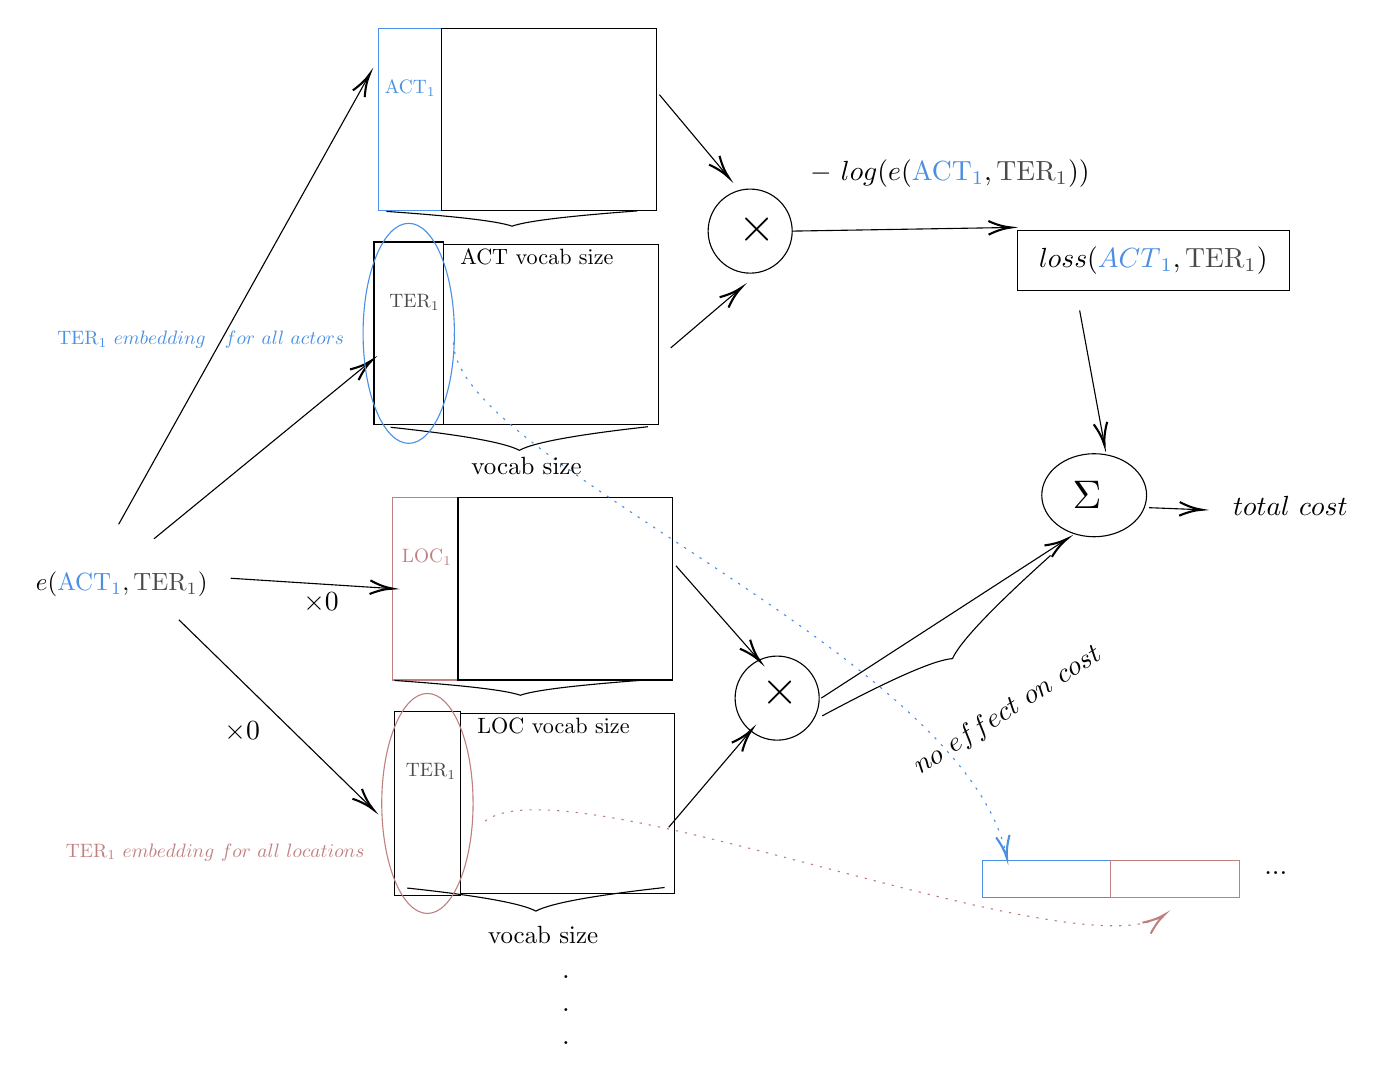
\begin{tikzpicture}[x=0.75pt,y=0.75pt,yscale=-1,xscale=1]
%uncomment if require: \path (0,547); %set diagram left start at 0, and has height of 547

%Straight Lines [id:da13430096728319052] 
\draw    (71.5,277) -- (174.95,192.27) ;
\draw [shift={(176.5,191)}, rotate = 500.68] [color={rgb, 255:red, 0; green, 0; blue, 0 }  ][line width=0.75]    (10.93,-3.29) .. controls (6.95,-1.4) and (3.31,-0.3) .. (0,0) .. controls (3.31,0.3) and (6.95,1.4) .. (10.93,3.29)   ;

%Straight Lines [id:da3395203365138022] 
\draw    (54.5,270) -- (174.53,54.75) ;
\draw [shift={(175.5,53)}, rotate = 479.14] [color={rgb, 255:red, 0; green, 0; blue, 0 }  ][line width=0.75]    (10.93,-3.29) .. controls (6.95,-1.4) and (3.31,-0.3) .. (0,0) .. controls (3.31,0.3) and (6.95,1.4) .. (10.93,3.29)   ;

%Shape: Rectangle [id:dp40988752111198234] 
\draw  [color={rgb, 255:red, 74; green, 144; blue, 226 }  ,draw opacity=1 ] (179.5,31) -- (210,31) -- (210,119) -- (179.5,119) -- cycle ;
%Shape: Rectangle [id:dp8120457242640955] 
\draw   (177.5,134) -- (211,134) -- (211,222) -- (177.5,222) -- cycle ;
%Shape: Rectangle [id:dp5994549314957651] 
\draw  [color={rgb, 255:red, 0; green, 0; blue, 0 }  ,draw opacity=1 ] (210,31) -- (313.5,31) -- (313.5,119) -- (210,119) -- cycle ;
%Shape: Rectangle [id:dp8953379233256253] 
\draw  [color={rgb, 255:red, 0; green, 0; blue, 0 }  ,draw opacity=1 ] (211,135) -- (314.5,135) -- (314.5,222) -- (211,222) -- cycle ;
\draw   (309.5,223) .. controls (275.06,226.82) and (254.4,230.61) .. (247.52,234.37) .. controls (240.63,230.64) and (219.95,226.93) .. (185.5,223.26) ;
\draw   (304.5,119) .. controls (270.9,121.49) and (250.73,123.94) .. (244.02,126.37) .. controls (237.29,123.97) and (217.12,121.6) .. (183.5,119.25) ;
%Shape: Ellipse [id:dp16021666171497673] 
\draw   (338.5,128.75) .. controls (338.5,117.57) and (347.57,108.5) .. (358.75,108.5) .. controls (369.93,108.5) and (379,117.57) .. (379,128.75) .. controls (379,139.93) and (369.93,149) .. (358.75,149) .. controls (347.57,149) and (338.5,139.93) .. (338.5,128.75) -- cycle ;
%Straight Lines [id:da010832594540308715] 
\draw    (320.5,185) -- (352.98,157.3) ;
\draw [shift={(354.5,156)}, rotate = 499.54] [color={rgb, 255:red, 0; green, 0; blue, 0 }  ][line width=0.75]    (10.93,-3.29) .. controls (6.95,-1.4) and (3.31,-0.3) .. (0,0) .. controls (3.31,0.3) and (6.95,1.4) .. (10.93,3.29)   ;

%Straight Lines [id:da7904695547993323] 
\draw    (315,63) -- (347.22,101.47) ;
\draw [shift={(348.5,103)}, rotate = 230.05] [color={rgb, 255:red, 0; green, 0; blue, 0 }  ][line width=0.75]    (10.93,-3.29) .. controls (6.95,-1.4) and (3.31,-0.3) .. (0,0) .. controls (3.31,0.3) and (6.95,1.4) .. (10.93,3.29)   ;

%Straight Lines [id:da40310566362864897] 
\draw    (517.5,167) -- (529.14,230.03) ;
\draw [shift={(529.5,232)}, rotate = 259.54] [color={rgb, 255:red, 0; green, 0; blue, 0 }  ][line width=0.75]    (10.93,-3.29) .. controls (6.95,-1.4) and (3.31,-0.3) .. (0,0) .. controls (3.31,0.3) and (6.95,1.4) .. (10.93,3.29)   ;

%Shape: Rectangle [id:dp7172146507008619] 
\draw  [color={rgb, 255:red, 191; green, 128; blue, 128 }  ,draw opacity=1 ] (186.5,257) -- (218,257) -- (218,345) -- (186.5,345) -- cycle ;
%Shape: Rectangle [id:dp060267406747659624] 
\draw   (187.5,360) -- (219,360) -- (219,449) -- (187.5,449) -- cycle ;
%Shape: Rectangle [id:dp6303673802072765] 
\draw  [color={rgb, 255:red, 0; green, 0; blue, 0 }  ,draw opacity=1 ] (218,257) -- (321.5,257) -- (321.5,345) -- (218,345) -- cycle ;
%Shape: Rectangle [id:dp304301296261714] 
\draw  [color={rgb, 255:red, 0; green, 0; blue, 0 }  ,draw opacity=1 ] (219,361) -- (322.5,361) -- (322.5,448) -- (219,448) -- cycle ;
\draw   (317.5,445) .. controls (283.06,448.82) and (262.4,452.61) .. (255.52,456.37) .. controls (248.63,452.64) and (227.95,448.93) .. (193.5,445.26) ;
%Shape: Ellipse [id:dp22428072345396544] 
\draw   (351.5,353.75) .. controls (351.5,342.57) and (360.57,333.5) .. (371.75,333.5) .. controls (382.93,333.5) and (392,342.57) .. (392,353.75) .. controls (392,364.93) and (382.93,374) .. (371.75,374) .. controls (360.57,374) and (351.5,364.93) .. (351.5,353.75) -- cycle ;
%Straight Lines [id:da29040700011246456] 
\draw    (319.5,416) -- (358.2,370.52) ;
\draw [shift={(359.5,369)}, rotate = 490.4] [color={rgb, 255:red, 0; green, 0; blue, 0 }  ][line width=0.75]    (10.93,-3.29) .. controls (6.95,-1.4) and (3.31,-0.3) .. (0,0) .. controls (3.31,0.3) and (6.95,1.4) .. (10.93,3.29)   ;

%Straight Lines [id:da7545042977801857] 
\draw    (323,290) -- (362.18,334.5) ;
\draw [shift={(363.5,336)}, rotate = 228.64] [color={rgb, 255:red, 0; green, 0; blue, 0 }  ][line width=0.75]    (10.93,-3.29) .. controls (6.95,-1.4) and (3.31,-0.3) .. (0,0) .. controls (3.31,0.3) and (6.95,1.4) .. (10.93,3.29)   ;

%Straight Lines [id:da13418076605656504] 
\draw    (393,353.75) -- (509.82,278.09) ;
\draw [shift={(511.5,277)}, rotate = 507.07] [color={rgb, 255:red, 0; green, 0; blue, 0 }  ][line width=0.75]    (10.93,-3.29) .. controls (6.95,-1.4) and (3.31,-0.3) .. (0,0) .. controls (3.31,0.3) and (6.95,1.4) .. (10.93,3.29)   ;

\draw   (308.5,345) .. controls (274.9,347.49) and (254.73,349.94) .. (248.02,352.37) .. controls (241.29,349.97) and (221.12,347.6) .. (187.5,345.25) ;
%Shape: Ellipse [id:dp1891084828946663] 
\draw  [color={rgb, 255:red, 74; green, 144; blue, 226 }  ,draw opacity=1 ] (172.25,178) .. controls (172.25,148.73) and (182.1,125) .. (194.25,125) .. controls (206.4,125) and (216.25,148.73) .. (216.25,178) .. controls (216.25,207.27) and (206.4,231) .. (194.25,231) .. controls (182.1,231) and (172.25,207.27) .. (172.25,178) -- cycle ;
%Shape: Ellipse [id:dp5133297466247488] 
\draw  [color={rgb, 255:red, 191; green, 128; blue, 128 }  ,draw opacity=1 ] (181.25,404.5) .. controls (181.25,375.23) and (191.1,351.5) .. (203.25,351.5) .. controls (215.4,351.5) and (225.25,375.23) .. (225.25,404.5) .. controls (225.25,433.77) and (215.4,457.5) .. (203.25,457.5) .. controls (191.1,457.5) and (181.25,433.77) .. (181.25,404.5) -- cycle ;
%Shape: Rectangle [id:dp8154703521346762] 
\draw  [color={rgb, 255:red, 74; green, 144; blue, 226 }  ,draw opacity=1 ] (470.5,432) -- (532.5,432) -- (532.5,450) -- (470.5,450) -- cycle ;
%Shape: Rectangle [id:dp3576905019222951] 
\draw  [color={rgb, 255:red, 191; green, 128; blue, 128 }  ,draw opacity=1 ] (532.5,432) -- (594.5,432) -- (594.5,450) -- (532.5,450) -- cycle ;
%Straight Lines [id:da3207889104512305] 
\draw    (108.5,296) -- (184.5,300.87) ;
\draw [shift={(186.5,301)}, rotate = 183.67] [color={rgb, 255:red, 0; green, 0; blue, 0 }  ][line width=0.75]    (10.93,-3.29) .. controls (6.95,-1.4) and (3.31,-0.3) .. (0,0) .. controls (3.31,0.3) and (6.95,1.4) .. (10.93,3.29)   ;

%Straight Lines [id:da444746435738554] 
\draw    (83.5,316) -- (175.82,406.1) ;
\draw [shift={(177.25,407.5)}, rotate = 224.3] [color={rgb, 255:red, 0; green, 0; blue, 0 }  ][line width=0.75]    (10.93,-3.29) .. controls (6.95,-1.4) and (3.31,-0.3) .. (0,0) .. controls (3.31,0.3) and (6.95,1.4) .. (10.93,3.29)   ;

\draw   (503.5,285) .. controls (475.52,310.16) and (459.77,326.73) .. (456.25,334.71) .. controls (447.55,335.32) and (426.62,344.52) .. (393.47,362.3) ;
%Shape: Ellipse [id:dp6408782289262511] 
\draw   (499.25,256) .. controls (499.25,244.95) and (510.55,236) .. (524.5,236) .. controls (538.45,236) and (549.75,244.95) .. (549.75,256) .. controls (549.75,267.05) and (538.45,276) .. (524.5,276) .. controls (510.55,276) and (499.25,267.05) .. (499.25,256) -- cycle ;
%Straight Lines [id:da19133214528940812] 
\draw    (379,128.75) -- (482.5,127.03) ;
\draw [shift={(484.5,127)}, rotate = 539.05] [color={rgb, 255:red, 0; green, 0; blue, 0 }  ][line width=0.75]    (10.93,-3.29) .. controls (6.95,-1.4) and (3.31,-0.3) .. (0,0) .. controls (3.31,0.3) and (6.95,1.4) .. (10.93,3.29)   ;

%Straight Lines [id:da406862365844594] 
\draw    (551,262) -- (574.5,262.92) ;
\draw [shift={(576.5,263)}, rotate = 182.25] [color={rgb, 255:red, 0; green, 0; blue, 0 }  ][line width=0.75]    (10.93,-3.29) .. controls (6.95,-1.4) and (3.31,-0.3) .. (0,0) .. controls (3.31,0.3) and (6.95,1.4) .. (10.93,3.29)   ;

%Curve Lines [id:da14396608756415818] 
\draw [color={rgb, 255:red, 191; green, 128; blue, 128 }  ,draw opacity=1 ] [dash pattern={on 0.84pt off 2.51pt}]  (231,413) .. controls (270.6,383.3) and (513.57,485.91) .. (557.24,458.86) ;
\draw [shift={(558.5,458)}, rotate = 503.13] [color={rgb, 255:red, 191; green, 128; blue, 128 }  ,draw opacity=1 ][line width=0.75]    (10.93,-3.29) .. controls (6.95,-1.4) and (3.31,-0.3) .. (0,0) .. controls (3.31,0.3) and (6.95,1.4) .. (10.93,3.29)   ;

%Curve Lines [id:da8005082280810756] 
\draw [color={rgb, 255:red, 74; green, 144; blue, 226 }  ,draw opacity=1 ] [dash pattern={on 0.84pt off 2.51pt}]  (216.25,178) .. controls (203.56,234.72) and (460.91,329.05) .. (482.2,429.49) ;
\draw [shift={(482.5,431)}, rotate = 259.35] [color={rgb, 255:red, 74; green, 144; blue, 226 }  ,draw opacity=1 ][line width=0.75]    (10.93,-3.29) .. controls (6.95,-1.4) and (3.31,-0.3) .. (0,0) .. controls (3.31,0.3) and (6.95,1.4) .. (10.93,3.29)   ;


% Text Node
\draw (195,60) node [scale=0.7,color={rgb, 255:red, 74; green, 144; blue, 226 }  ,opacity=1 ]  {$\mathrm{ACT}_{1}$};
% Text Node
\draw (362,128) node [scale=1.7280000000000002]  {$\times $};
% Text Node
\draw (197,163) node [scale=0.7,color={rgb, 255:red, 74; green, 74; blue, 74 }  ,opacity=1 ]  {$\mathrm{TER}_{1}$};
% Text Node
\draw (256,141) node [scale=0.8] [align=left] {ACT vocab size};
% Text Node
\draw (251,242) node [scale=0.9] [align=left] {vocab size};
% Text Node
\draw (203,286) node [scale=0.7,color={rgb, 255:red, 191; green, 128; blue, 128 }  ,opacity=1 ]  {$\mathrm{LOC}_{1}$};
% Text Node
\draw (205,389) node [scale=0.7,color={rgb, 255:red, 74; green, 74; blue, 74 }  ,opacity=1 ]  {$\mathrm{TER}_{1}$};
% Text Node
\draw (264,367) node [scale=0.8] [align=left] {LOC vocab size};
% Text Node
\draw (259,468) node [scale=0.9] [align=left] {vocab size};
% Text Node
\draw (270,504) node  [align=left] {.\\.\\.};
% Text Node
\draw (94,181) node [scale=0.7,color={rgb, 255:red, 74; green, 144; blue, 226 }  ,opacity=1 ]  {$\mathrm{TER}_{1} \ embedding\ \ \ for\ all\ actors$};
% Text Node
\draw (101,428) node [scale=0.7,color={rgb, 255:red, 191; green, 128; blue, 128 }  ,opacity=1 ]  {$\mathrm{TER}_{1} \ embedding\ for\ all\ locations$};
% Text Node
\draw (612,438) node  [align=left] {...};
% Text Node
\draw (114,370) node   {$\times 0$};
% Text Node
\draw (152,308) node   {$\times 0$};
% Text Node
\draw (483,360) node [rotate=-327.48]  {$ \begin{array}{l}
no\ effect\ on\ cost\\
\end{array}$};
% Text Node
\draw (521,256) node [scale=1.44]  {$\Sigma $};
% Text Node
\draw (373,351) node [scale=1.7280000000000002]  {$\times $};
% Text Node
\draw (56,299) node [scale=0.9] [align=left] {$e (\textcolor[rgb]{0.29,0.56,0.89}{\mathrm{ACT}}\textcolor[rgb]{0.29,0.56,0.89}{_{1}} ,\textcolor[rgb]{0.29,0.29,0.29}{\mathrm{TER}_{1}})$};
% Text Node
\draw    (487.5,128.5) -- (618.5,128.5) -- (618.5,157.5) -- (487.5,157.5) -- cycle  ;
\draw (553,143) node  [align=left] {$loss(\textcolor[rgb]{0.29,0.56,0.89}{ACT}\textcolor[rgb]{0.29,0.56,0.89}{_{1}} ,\textcolor[rgb]{0.29,0.29,0.29}{\mathrm{TER}_{1}})$};
% Text Node
\draw (455,101) node  [align=left] {$-\ log( e (\textcolor[rgb]{0.29,0.56,0.89}{\mathrm{ACT}}\textcolor[rgb]{0.29,0.56,0.89}{_{1}} ,\textcolor[rgb]{0.29,0.29,0.29}{\mathrm{TER}_{1}}))$};
% Text Node
\draw (619,261) node  [align=left] {$total\ cost$};


\end{tikzpicture}
\caption{Faceted embedding with unified cost function. Training for a single input is shown using only one network. The target word is TER$_1$, which is being trained against all actors, organisations, locations, dates and terms. While training, the weights related to actors are only updated if the input edge weight has the start node type of an actor. Meanwhile, the rest of the weights related to other entity-types are freezed. The final embedding is created by concatenating the columns in the context embedding matrices that are associated with TER$_1$.} \label{fig:unified_cost}
}
\end{figure}
 %%%%%%%%%%%%%%%%%%%%%%%%%%%%%%%%%%%%%%%%%%%%%%%%%%%%%%%%%%%%
  %%%%%%%%%%%%%%%%%%%%%%%%%%%%%%%%%%%%%%%%%%%%%%%%%%%%%%%%%%%%
\subsection{Vectorized faceted embeddings}
In order to speed up the model and use batch gradient descent we need to vectorize the cost function. In the following we go through the vectorization process for the embeddings with separate costs. The same idea can also be applied during the training of the unified cost function.\\
If we consider $W$ as the matrix of all focal embeddings and $\tilde{ W }$ as the matrix of all context embeddings stacked row-wise, then we can vectorize the model according to Equation~\ref{eq:vectorized}. 
\begin{equation}
J=(W \hat{  W }^{ \top } +B+\tilde{ B } -log{ X })^{ 2 }
\label{eq:vectorized}
\end{equation}
%The original GloVe model contains:
%\begin{itemize}
%\item $W \in R^{V \times M} $ for focal embeddings.
% \item $\tilde{ W }  \in R^{V \times M} $ for context embeddings.
%\item $B,\tilde{B} \in R^{V \times 1}$ biases for focal and context embeddings. 
%\item $X \in R^{V\times V} $ co-occurrence matrix of the whole vocabulary. 
%\end{itemize}
Unlike the original GloVe model, the dimensions of  $W$ and $\tilde{ W } $ are no longer equal as our weighted adjacency matrix is no longer symmetric $X \in R^{|V_f|\times |V|} $.  $V_f$ is the set of all focal words, which is defined by the input. If actors are the focal words then $V_f$ is the  of all actors in the vocabulary. The parameters of the model are as follows: 
\begin{itemize}
\item $W \in R^{|V_f| \times M} $ for focal embeddings.
 \item $\tilde{ W }  \in R^{|V| \times M} $ for context embeddings.
\item $B,\tilde{B} \in R^{|V_f| \times 1}$ biases for focal and context embeddings.
\item $X \in R^{|V_f|\times |V|} $ co-occurrence matrix of the whole vocabulary. 
\end{itemize}
Biases have to be added row-wise to the matrices to preserve the original cost function~\ref{eq:glove_cost}. As a consequence, they are transformed to column vectors in the size of the focal vocabulary. A visual comparison between the original GloVe model ($J_g$) and our faceted cost function ($J_f$) can be seen below, where the size of the vocabulary is indicated by $|V|=v$ and size of the focal vocabulary by $|V_f|=v_f$\\
\[J_{f}=\stackrel{\mbox{$W(v\times M)$ }}{%
    \begin{bmatrix}
    a_{11} & a_{12}  \cdots  a_{1M} \\
    a_{21} & a_{22}  \cdots  a_{2M} \\
    \vdots & \vdots  \ddots  \vdots \\
    a_{v1} & a_{v2}  \cdots  a_{vM}
    \end{bmatrix}%
  } .
  \stackrel{\mbox{$\tilde{W}^T(M \times v)$ }}{%
    \begin{bmatrix}
    a_{11} & a_{12}  \cdots  a_{1v} \\
    a_{21} & a_{22}  \cdots  a_{2v} \\
    \vdots & \vdots  \ddots  \vdots \\
    a_{M1} & a_{M2}  \cdots  a_{Mv}
    \end{bmatrix}%
  } +
  \stackrel{B( v \times 1)}{%
    \begin{bmatrix}
    e_1 \\
    e_2 \\
    \vdots \\
    e_{v}
    \end{bmatrix}%
   }
   +
  \stackrel{\tilde{B |V|\times 1)}}{%
    \begin{bmatrix}
    e_1 \\
    e_2 \\
    \vdots \\
    e_{v}
    \end{bmatrix}%
   }-
   \stackrel{\mbox{$logX(v \times v)$ }}{%
    \begin{bmatrix}
    a_{11} & a_{12}  \cdots  a_{1v} \\
    a_{21} & a_{22}  \cdots  a_{2v} \\
    \vdots & \vdots  \ddots  \vdots \\
    a_{v1} & a_{v2}  \cdots  a_{vv}
    \end{bmatrix}%
  }
\]
\\
\[J_{f} =\stackrel{\mbox{$W( v_{f}\times M)$ }}{%
    \begin{bmatrix}
    a_{11} & a_{12}  \cdots  a_{1M} \\
    a_{21} & a_{22}  \cdots  a_{2M} \\
    \vdots & \vdots  \ddots  \vdots \\
    a_{v1} & a_{v2}  \cdots  a_{v
_{e}M}
    \end{bmatrix}%
  } .
  \stackrel{\mbox{$\tilde{W}^T(M \times |V|)$ }}{%
    \begin{bmatrix}
    a_{11} & a_{12}  \cdots  a_{1v} \\
    a_{21} & a_{22} \cdots  a_{2v} \\
    \vdots & \vdots \ddots \vdots \\
    a_{M1} & a_{M2}  \cdots  a_{Mv}
    \end{bmatrix}%
  } +
  \stackrel{B( v_{f}\times 1)}{%
    \begin{bmatrix}
    e_1 \\
    e_2 \\
    \vdots \\
    e_{v_{f}}
    \end{bmatrix}%
   }
   +
  \stackrel{\tilde{B}(v_{f}\times 1)}{%
    \begin{bmatrix}
    e_1 \\
    e_2 \\
    \vdots \\
    e_{v_{f}}
    \end{bmatrix}%
   }-
   \stackrel{\mbox{$logX( v_{f}\ \times v)$ }}{%
    \begin{bmatrix}
    a_{11} & a_{12}  \cdots  a_{1v} \\
    a_{21} & a_{22}  \cdots  a_{2v} \\
    \vdots & \vdots  \ddots  \vdots \\
    a_{v1} & a_{v2}  \cdots  a_{v_{f}v}
    \end{bmatrix}%
  }
\]

\section{Faceted Word2vec}\label{sec:faceted_word2vec}
Word embeddings are used as input features in many NLP tasks. Although methods like word2vec capture semantic features well, they often lack task-specific features. Thus, many studies focus on modifying and tweaking the existing methods for certain tasks, such as text classification~\brackettext{\cite{DBLP:conf/coling/LiuHGWTL18}}, semantic relation classification~\brackettext{\cite{DBLP:conf/conll/HashimotoSMT15}} and dependency parsing~\brackettext{\cite{DBLP:conf/acl/BansalGL14}}. Since with faceted embedding we also aim to modify existing methods to match our specific task, we looked a wide range of litreture on modifications of word embedding methods. In $2014$, Levy and Goldberg proposed a method to generalize the skip-gram achitecure of word2vec to include arbitrary contexts and used it to create dependency based embeddings~\brackettext{\cite{DBLP:conf/acl/LevyG14}}. We use the idea behind this model to define our own context for the skip-gram model, which allows us to learn the separate components of the faceted embedding. In this section, first, we give a brief description of embeddings with arbitrary contexts by Levy and Goldberg. Then, we look at our definition of context and modifications to the original model. Finally, we use this knowledge to generate the algorithm faceted word2vec. The model proposed by Levy and Goldberg uses the skip-gram architecture, thus, we also generate the faceted word2vec based on skip-gram and do not use the CBOW architecture.\\
For creating the faceted model using embeddings with arbitrary contexts, we follow these four steps: 
\begin{enumerate}        
 \item Extraction of type-specific edge lists from the co-occurrence graph, discussed in Section~\ref{sec:edges_as_pairs}.
 \item Training a low dimensional embedding for each edge list using the method proposed by  Levy and Goldberg, where the focal context pairs are edges of the graph~\brackettext{\cite{DBLP:conf/acl/LevyG14}}, discussed in Section~\ref{sec:arbitarty_context}.
 \item Disregarding the focal embeddings and keeping only the context embeddings, as it represents the relation of a word to entities of a specific type. 
 \item Concatenating the context embedding of all types to create the final embedding. 
 \end{enumerate}
 %%%%%%%%%%%%%%%%%%%%%%%%%%%%%%%%%%%%%%%%%%%%%%%%%%%%%%%%%%%%
\subsection{Embeddings with arbitrary contexts}\label{sec:arbitarty_context}
The general principle behind skip-gram is to bring words that appear in similar contexts in the text, closer in embedding space, where the contexts of a word are the words surrounding it. Therefore, the context vocabulary $C$ is identical to the complete word vocabulary $V$. In other words, the focal words and their context share the same vocabulary. Nonetheless, for embeddings with arbitrary contexts, this restriction is not required. The context does not need to correspond to words and can be defined based on the use-case, which is an important attribute for the faceted model. The negative sampling objective of word2vec, shown in Equation~\ref{eq:w2v_negative}, assumes a dataset $Q$ of focal and context pairs $(f,c)$ from a large body of text and samples negative examples form $\overline{Q}$. The model assigns a low score to the random negative samples and a high score to the real focal and context pairs. Since the input of the model is word pairs, it can be constructed in an arbitrary way. Levy and Goldberg specifically look at contexts, based on the syntactic relations, where the context is defined by the type of the dependency relation between the head and the modifier. They scan the text once and create focal and context pairs based on specific dependency relations and then use the generated pairs as positive inputs. For each $(f,c) \in Q$, $n$ samples $(f,c_1),\dots,(f,c_n)$ are constructed as negative examples, where $c_j$ is drawn according to its unigram distribution raised to the power of $\frac{3}{4}$~\brackettext{\cite{DBLP:conf/acl/LevyG14}}. Their framework is not only limited to dependency relations but also allows for various context definitions\cite{SCHOL:website/Levy2014}. Following their example, we can define a type-specific context to generate faceted embeddings. We denoted the faceted word2vec model by $f$W2V, where $f$ indicates the faceted model. In the following section, we show how the edges of co-occurrence graphs are used as focal and context pairs for our study.
 %%%%%%%%%%%%%%%%%%%%%%%%%%%%%%%%%%%%%%%%%%%%%%%%%%%%%%%%%%%%
\subsection{Edges of co-occurrence graphs as focal and context pairs}\label{sec:edges_as_pairs}
We take advantage of the definition of arbitrary context and define our context based on the types of entities surrounding a word. Our goal is to create embeddings, such that each part corresponds to the word related to the specific type of entities and a co-occurrence graph extracted from annotated text can help us achieve just that. To obtain each part of the embedding we define a type-specific edge list, in a similar fashion as type-specific adjacency matrices for faceted GloVe, where the start nodes are entities of a specific type and end nodes can be any term or entity from the vocabulary. More formally, in the heterogeneous graph $G=(V,E)$, where $V=A\bigcup  L\bigcup  \bigcup  O\bigcup  D\bigcup T $ is the set of all nodes with types actors, locations, organisations, dates, and any non-entity word (term) and $E$ is the set of all weighted edges, we extract the edge list where the start node is one of the types in set $V$. An example of the edge lists is shown in Figure~\ref{fig:facettedword2vec}. As demonstrated in Figure~\ref{fig:facettedword2vec}, we have a different edge list for each type. These edge lists can be treated as a focal and context pairs $(f,c)$ for the input of embeddings with arbitrary contexts, where $c \in V$ and $a$ is a specific type, e.g, $f \in A$ for generating actor part of the embedding. Thus, the focal and context vocabulary are not equal, as the focal vocabulary is always a subset of the context ($A \subset  V$). 
\begin{figure}
\centering 
\resizebox{0.80\textwidth}{0.28\textwidth}{      
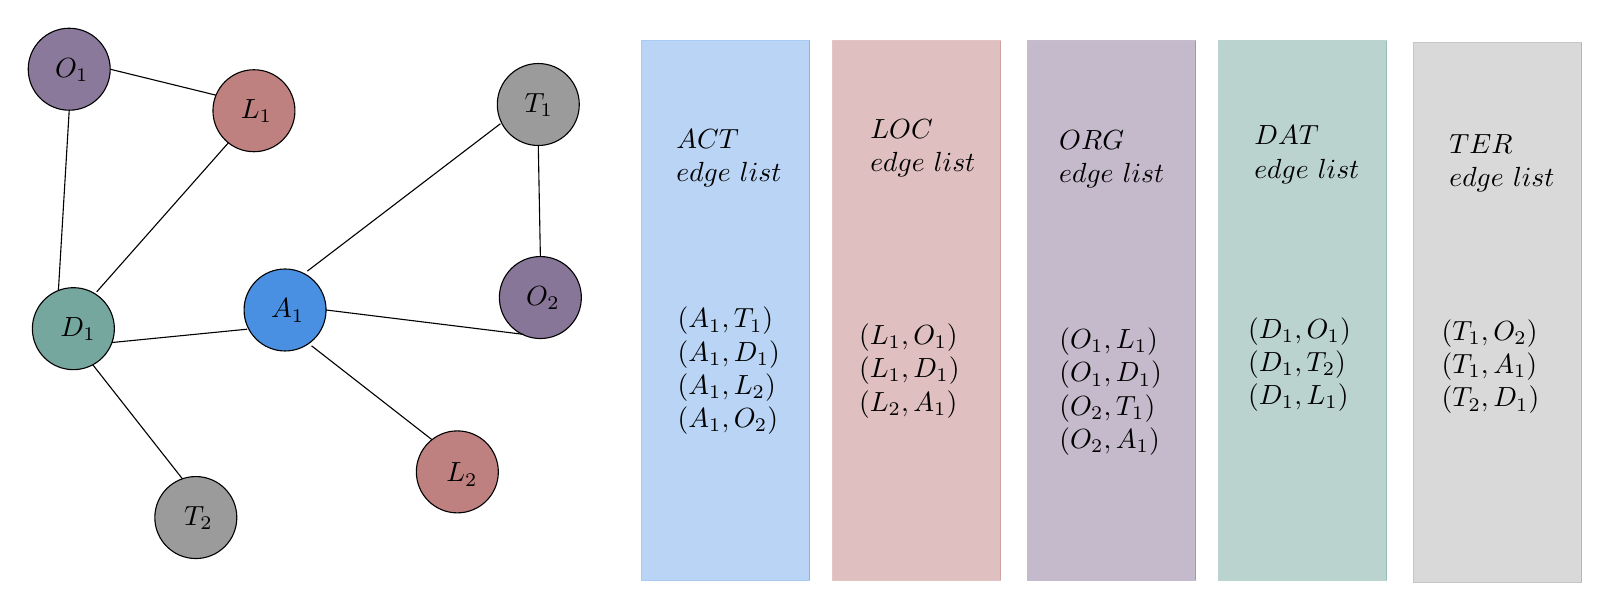
\begin{tikzpicture}[x=0.75pt,y=0.75pt,yscale=-1,xscale=1]
%uncomment if require: \path (0,324); %set diagram left start at 0, and has height of 324

%Shape: Circle [id:dp7723989663764896] 
\draw  [fill={rgb, 255:red, 120; green, 99; blue, 139 }  ,fill opacity=0.86 ] (24,56.75) .. controls (24,45.84) and (32.84,37) .. (43.75,37) .. controls (54.66,37) and (63.5,45.84) .. (63.5,56.75) .. controls (63.5,67.66) and (54.66,76.5) .. (43.75,76.5) .. controls (32.84,76.5) and (24,67.66) .. (24,56.75) -- cycle ;
%Straight Lines [id:da631891041159494] 
\draw    (269.75,93.5) -- (270.75,147) ;


%Straight Lines [id:da4375886533634059] 
\draw    (63.5,56.75) -- (117.5,70) ;


%Straight Lines [id:da6613925859828091] 
\draw    (121.5,91) -- (57,164) ;


%Straight Lines [id:da39535906402000176] 
\draw    (129.5,182) -- (58.5,189) ;


%Straight Lines [id:da6929421363539265] 
\draw    (55,199) -- (104.5,262) ;


%Straight Lines [id:da7460610286620943] 
\draw    (160.5,190) -- (219.5,236) ;


%Straight Lines [id:da9790672124174229] 
\draw    (251.5,83) -- (158.5,154) ;


%Straight Lines [id:da63778288309677] 
\draw    (38.5,164) -- (43.75,76.5) ;


%Shape: Circle [id:dp5787703304890821] 
\draw  [fill={rgb, 255:red, 117; green, 167; blue, 159 }  ,fill opacity=1 ] (26,181.75) .. controls (26,170.84) and (34.84,162) .. (45.75,162) .. controls (56.66,162) and (65.5,170.84) .. (65.5,181.75) .. controls (65.5,192.66) and (56.66,201.5) .. (45.75,201.5) .. controls (34.84,201.5) and (26,192.66) .. (26,181.75) -- cycle ;
%Shape: Circle [id:dp2977758613059365] 
\draw  [fill={rgb, 255:red, 191; green, 128; blue, 128 }  ,fill opacity=1 ] (113,76.75) .. controls (113,65.84) and (121.84,57) .. (132.75,57) .. controls (143.66,57) and (152.5,65.84) .. (152.5,76.75) .. controls (152.5,87.66) and (143.66,96.5) .. (132.75,96.5) .. controls (121.84,96.5) and (113,87.66) .. (113,76.75) -- cycle ;
%Shape: Circle [id:dp8211852276895382] 
\draw  [fill={rgb, 255:red, 74; green, 144; blue, 226 }  ,fill opacity=1 ] (128,172.75) .. controls (128,161.84) and (136.84,153) .. (147.75,153) .. controls (158.66,153) and (167.5,161.84) .. (167.5,172.75) .. controls (167.5,183.66) and (158.66,192.5) .. (147.75,192.5) .. controls (136.84,192.5) and (128,183.66) .. (128,172.75) -- cycle ;
%Shape: Circle [id:dp7755720350359876] 
\draw  [fill={rgb, 255:red, 155; green, 155; blue, 155 }  ,fill opacity=1 ] (85,272.75) .. controls (85,261.84) and (93.84,253) .. (104.75,253) .. controls (115.66,253) and (124.5,261.84) .. (124.5,272.75) .. controls (124.5,283.66) and (115.66,292.5) .. (104.75,292.5) .. controls (93.84,292.5) and (85,283.66) .. (85,272.75) -- cycle ;
%Shape: Circle [id:dp8914724887147505] 
\draw  [fill={rgb, 255:red, 155; green, 155; blue, 155 }  ,fill opacity=1 ] (250,73.75) .. controls (250,62.84) and (258.84,54) .. (269.75,54) .. controls (280.66,54) and (289.5,62.84) .. (289.5,73.75) .. controls (289.5,84.66) and (280.66,93.5) .. (269.75,93.5) .. controls (258.84,93.5) and (250,84.66) .. (250,73.75) -- cycle ;
%Shape: Circle [id:dp06424977358736528] 
\draw  [fill={rgb, 255:red, 191; green, 128; blue, 128 }  ,fill opacity=1 ] (211,250.75) .. controls (211,239.84) and (219.84,231) .. (230.75,231) .. controls (241.66,231) and (250.5,239.84) .. (250.5,250.75) .. controls (250.5,261.66) and (241.66,270.5) .. (230.75,270.5) .. controls (219.84,270.5) and (211,261.66) .. (211,250.75) -- cycle ;
%Shape: Circle [id:dp5224682342118112] 
\draw  [fill={rgb, 255:red, 120; green, 99; blue, 139 }  ,fill opacity=0.88 ] (251,166.75) .. controls (251,155.84) and (259.84,147) .. (270.75,147) .. controls (281.66,147) and (290.5,155.84) .. (290.5,166.75) .. controls (290.5,177.66) and (281.66,186.5) .. (270.75,186.5) .. controls (259.84,186.5) and (251,177.66) .. (251,166.75) -- cycle ;
%Straight Lines [id:da168907494889315] 
\draw    (262.75,184.5) -- (167.5,172.75) ;


%Shape: Rectangle [id:dp4597340173200979] 
\draw  [color={rgb, 255:red, 74; green, 144; blue, 226 }  ,draw opacity=0.47 ][fill={rgb, 255:red, 74; green, 144; blue, 226 }  ,fill opacity=0.39 ] (319.5,43) -- (400.5,43) -- (400.5,303) -- (319.5,303) -- cycle ;
%Shape: Rectangle [id:dp8236283831060471] 
\draw  [color={rgb, 255:red, 191; green, 128; blue, 128 }  ,draw opacity=0.46 ][fill={rgb, 255:red, 191; green, 128; blue, 128 }  ,fill opacity=0.5 ] (411.5,43) -- (492.5,43) -- (492.5,303) -- (411.5,303) -- cycle ;
%Shape: Rectangle [id:dp9350536299021817] 
\draw  [color={rgb, 255:red, 120; green, 99; blue, 139 }  ,draw opacity=0.43 ][fill={rgb, 255:red, 120; green, 99; blue, 139 }  ,fill opacity=0.44 ] (505.5,43) -- (586.5,43) -- (586.5,303) -- (505.5,303) -- cycle ;
%Shape: Rectangle [id:dp287143176572378] 
\draw  [color={rgb, 255:red, 117; green, 167; blue, 159 }  ,draw opacity=0.49 ][fill={rgb, 255:red, 117; green, 167; blue, 159 }  ,fill opacity=0.5 ] (597.5,43) -- (678.5,43) -- (678.5,303) -- (597.5,303) -- cycle ;
%Shape: Rectangle [id:dp42566484032417296] 
\draw  [color={rgb, 255:red, 155; green, 155; blue, 155 }  ,draw opacity=0.57 ][fill={rgb, 255:red, 155; green, 155; blue, 155 }  ,fill opacity=0.38 ] (691.5,44) -- (772.5,44) -- (772.5,304) -- (691.5,304) -- cycle ;

% Text Node
\draw (45,57) node   {$O_{1}$};
% Text Node
\draw (48,182) node   {$D_{1}$};
% Text Node
\draw (134,77) node   {$L_{1}$};
% Text Node
\draw (149,173) node   {$A_{1}$};
% Text Node
\draw (106,273) node   {$T_{2}$};
% Text Node
\draw (270,74) node   {$T_{1}$};
% Text Node
\draw (233,252) node   {$L_{2}$};
% Text Node
\draw (272,167) node   {$O_{2}$};
% Text Node
\draw (361.56,99.77) node   {$ \begin{array}{l}
ACT\ \\
edge\ list
\end{array}$};
% Text Node
\draw (455,95) node   {$ \begin{array}{l}
LOC\ \\
edge\ list
\end{array}$};
% Text Node
\draw (546,100) node   {$ \begin{array}{l}
ORG\ \\
edge\ list
\end{array}$};
% Text Node
\draw (640,98) node   {$ \begin{array}{l}
DAT\\
edge\ list
\end{array}$};
% Text Node
\draw (734,102) node   {$ \begin{array}{l}
TER\ \\
edge\ list
\end{array}$};
% Text Node
\draw (361.52,202.22) node   {$ \begin{array}{l}
( A_{1} ,T_{1})\\
( A_{1} ,D_{1})\\
( A_{1} ,L_{2})\\
( A_{1} ,O_{2})
\end{array}$};
% Text Node
\draw (448.52,210.22) node   {$ \begin{array}{l}
( L_{1} ,O_{1})\\
( L_{1} ,D_{1})\\
( L_{2} ,A_{1})\\
\\
\end{array}$};
% Text Node
\draw (545.52,220.22) node   {$ \begin{array}{l}
( O_{1} ,L_{1})\\
( O_{1} ,D_{1})\\
( O_{2} ,T_{1})\\
( O_{2} ,A_{1})\\
\\
\end{array}$};
% Text Node
\draw (636.52,207.22) node   {$ \begin{array}{l}
( D_{1} ,O_{1})\\
( D_{1} ,T_{2})\\
( D_{1} ,L_{1})\\
\\
\end{array}$};
% Text Node
\draw (728.52,208.22) node   {$ \begin{array}{l}
( T_{1} ,O_{2})\\
( T_{1} ,A_{1})\\
( T_{2} ,D_{1})\\
\\
\end{array}$};


\end{tikzpicture}
}
\caption{An example of creating type specific edge lists for a graph with node type: actor (A), location (L), organisation (L), date (D), and term (T).}
\label{fig:facettedword2vec}
\end{figure} 
Based on each edge list the model learns a separate embedding, with entities of a certain type as focal words and the rest of the vocabulary as context. As a result, each context embedding encodes the relation of the complete vocabulary with a certain type. For example, if we look at the context embedding for actors, it encodes the relation of the words in the vocabulary to all the actors. Naturally, if a word does not have an edge to any actor it will not be present in the context embeddings. For such cases, it makes sense to set the actor part of that word equal to a vector of zeros. For example, in Figure~\ref{fig:facettedword2vec}, $T_2$ will only have a non-zero date component and the rest are set to zero. This approach has some drawbacks, as the cosine similarity between a vector of zero and any other vector is undefined. Therefore, if a component of a vector is set to zero, that word becomes incomparable to all other words in that sub-space. It also causes  problems for clustering algorithms that require a distance measure between the points, if the cosine similarity is undefined, then we are unable to compare the words and form clusters. To solve this issue, we add a small number $0.0001$ to the vectors of all zero, mapping all the words to the same point, while keeping the component small. Moreover, clustering algorithms are able to compute the distance between the word vectors in the sub-spaces.This approach also has some unwanted implications,  if components of two word are identical, their cosine similarity is always one. Thus, any point that does not have relations to entities of a particular type are considered similar in that subspace, which is not always the case. For example, in Figure~\ref{fig:facettedword2vec}, $T_2$ and $L_2$ both have the same organisation component, as they are not connected to any organisation node. The absence of an edge to a organisation does not necessary mean that $T_2$ and $L_2$ should be similar in organisation space, which is what the model would imply. 
 %%%%%%%%%%%%%%%%%%%%%%%%%%%%%%%%%%%%%%%%%%%%%%%%%%%%%%%%%%%%

 %%%%%%%%%%%%%%%%%%%%%%%%%%%%%%%%%%%%%%%%%%%%%%%%%%%%%%%%%%%%
\section{Faceted DeepWalk}\label{sec:faceted_deepwalk}
Another way to achieve the faceted model is by taking advantage of the type-restricted random walks. For this purpose, we alter the DeepWalk model to meet our needs. In $2017$, \emph{metapath2vec} was proposed by Dong et al. to study representation learning in heterogeneous graphs with multiple edge and node types, such as coauthor relationships graphs~\brackettext{\cite{DBLP:conf/kdd/DongCS17}}. Metapath2vec learns a low dimensional representation of the graph using random walks that are restricted to the only transition between particular types of nodes and edges. They also introduce a heterogeneous skip-gram which maximizes the probability of having the heterogeneous context for a given node~\brackettext{\cite{DBLP:journals/tkde/CaiZC18}}. For learning the faceted embeddings, however, we take a more straightforward approach. We take advantage of the weighted random walks used in Chapter~\ref{chap:entity} to generate entity embeddings to introduce a new type-restricted random walk to restrict the context of a word to certain entity type. 
In general, faceted DeepWalk model consists of three steps: 
\begin{enumerate}
\item Generating type specific corpus based on type-restricted fixed length random walks starting from all the nodes in the graphs.
\item Applying the skip-gram model on the random walk corpora. 
\item Concatenating the resulting embedding for each type to achieve the final faceted model.  
\end{enumerate}
\emph{Type-restricted random walk:} Formally, a type-restricted random walk in graph $G=(V,E)$ is denoted in the form of $v_1 \rightarrow v_2 \rightarrow v_3\rightarrow \dots \rightarrow t_n$, where the nodes $t_i$ belong to a certain node type. In a graph, where $V=A\bigcup  L\bigcup  O\bigcup  D\bigcup  T$, to sample only locations related to a node, we perform a location-restricted random walk. Consequently, the transition probability for the restricted type $L$ between node $i$ and $j$ in a weighted graph is defined in Equation ~\ref{eq:transition_type_restricted}, where $e_{i,j}$ is the edge weight between the two nodes $i$ and $j$. Given that we are removing the possibility of transitioning to any type other than the pre-defined one, the probabilities are normalized by the summation of the edge weight of the pre-defined type.
\begin{equation}
P_{ i,j }=\left\{ 
\begin{matrix}
 \frac { f(e_{ i,j }) }{ \sum _{ k\in L,f(e_{ k })\in E_{ i } }^{  }{ f(e_{ k }) }  }  & \mathrm{if}\quad j\in L \\
0 & \mathrm{if}\quad j\notin L
\end{matrix} 
\right. 
\label{eq:transition_type_restricted}
\end{equation} 
\noindent
Function $f$ is the edge normalization function. Like entity embeddings, we use two normalization functions: \\
\begin{enumerate}
\item  $f=\mathrm{id}$, identity function. We denote these models by $f$DW$_{id}$, where $id$ shows the identity mapping. \\
\item  $f=\log$, logarithmic normalization. These models are denoted by  $f$DW$_{log}$.\\
\end{enumerate}
\noindent
An example of the type-restricted random walk for type location is illustrated in Figure~\ref{fig:facetteddeepwalk}. Any nodes in the random walk have to be a location to be visited, otherwise, it is disregard. Hence, by creating a type specific corpus with the type-restricted random walk, we can train a skip-gram model that learns the representation of all nodes with regards to a single entity type. By repeating this process for all node types and concatenating the results we achieve the faceted model.
\begin{figure}
\centering 
\resizebox{0.60\textwidth}{0.27\textwidth}{      
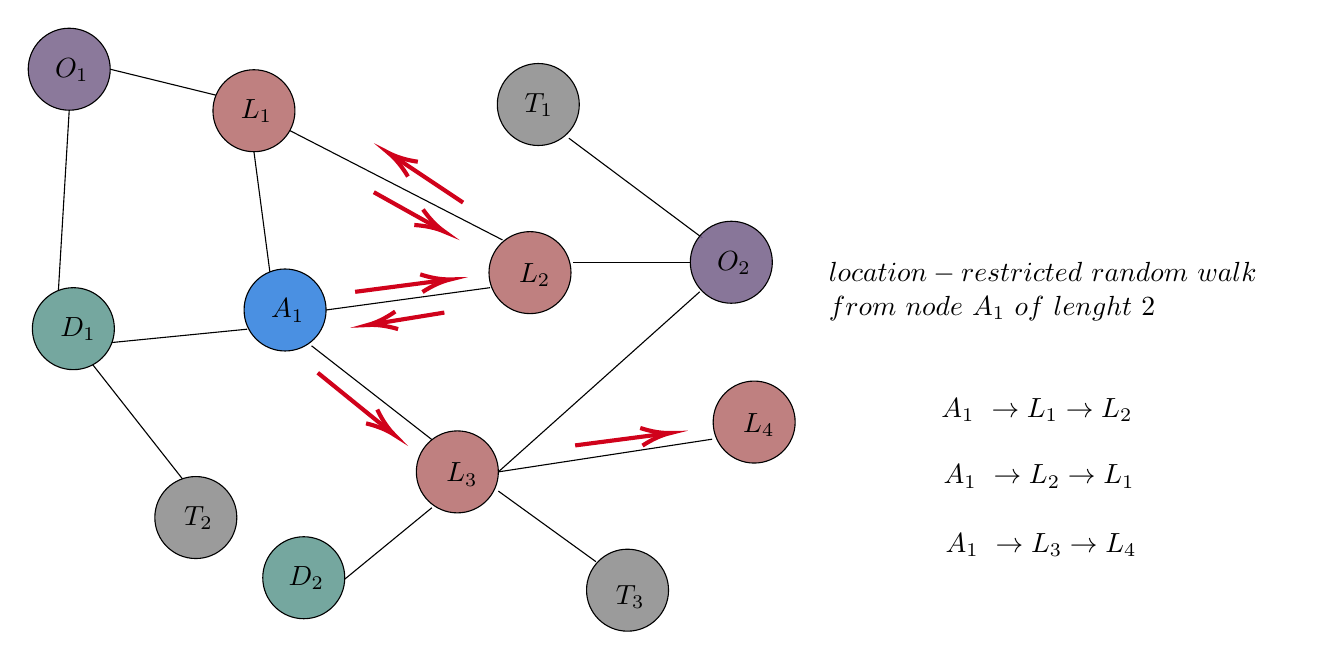
\begin{tikzpicture}[x=0.75pt,y=0.75pt,yscale=-1,xscale=1]
%uncomment if require: \path (0,424); %set diagram left start at 0, and has height of 424

%Shape: Circle [id:dp7408051866775183] 
\draw  [fill={rgb, 255:red, 120; green, 99; blue, 139 }  ,fill opacity=0.86 ] (25,44.75) .. controls (25,33.84) and (33.84,25) .. (44.75,25) .. controls (55.66,25) and (64.5,33.84) .. (64.5,44.75) .. controls (64.5,55.66) and (55.66,64.5) .. (44.75,64.5) .. controls (33.84,64.5) and (25,55.66) .. (25,44.75) -- cycle ;
%Straight Lines [id:da23542430963110572] 
\draw    (285.5,78) -- (349.75,126) ;


%Straight Lines [id:da9464008253728087] 
\draw    (64.5,44.75) -- (118.5,58) ;


%Straight Lines [id:da08217413408429564] 
\draw    (133.75,84.5) -- (141.5,143) ;


%Straight Lines [id:da09323667666851287] 
\draw    (130.5,170) -- (59.5,177) ;


%Straight Lines [id:da7962118124877697] 
\draw    (56,187) -- (105.5,250) ;


%Straight Lines [id:da5871309233503423] 
\draw    (161.5,178) -- (220.5,224) ;


%Straight Lines [id:da34174484678938555] 
\draw    (253.5,127) -- (148.5,73) ;


%Straight Lines [id:da666737517633426] 
\draw    (39.5,152) -- (44.75,64.5) ;


%Shape: Circle [id:dp2508008248936129] 
\draw  [fill={rgb, 255:red, 117; green, 167; blue, 159 }  ,fill opacity=1 ] (27,169.75) .. controls (27,158.84) and (35.84,150) .. (46.75,150) .. controls (57.66,150) and (66.5,158.84) .. (66.5,169.75) .. controls (66.5,180.66) and (57.66,189.5) .. (46.75,189.5) .. controls (35.84,189.5) and (27,180.66) .. (27,169.75) -- cycle ;
%Shape: Circle [id:dp4060574393112093] 
\draw  [fill={rgb, 255:red, 191; green, 128; blue, 128 }  ,fill opacity=1 ] (114,64.75) .. controls (114,53.84) and (122.84,45) .. (133.75,45) .. controls (144.66,45) and (153.5,53.84) .. (153.5,64.75) .. controls (153.5,75.66) and (144.66,84.5) .. (133.75,84.5) .. controls (122.84,84.5) and (114,75.66) .. (114,64.75) -- cycle ;
%Shape: Circle [id:dp36486264653360756] 
\draw  [fill={rgb, 255:red, 74; green, 144; blue, 226 }  ,fill opacity=1 ] (129,160.75) .. controls (129,149.84) and (137.84,141) .. (148.75,141) .. controls (159.66,141) and (168.5,149.84) .. (168.5,160.75) .. controls (168.5,171.66) and (159.66,180.5) .. (148.75,180.5) .. controls (137.84,180.5) and (129,171.66) .. (129,160.75) -- cycle ;
%Shape: Circle [id:dp08674187749849449] 
\draw  [fill={rgb, 255:red, 155; green, 155; blue, 155 }  ,fill opacity=1 ] (86,260.75) .. controls (86,249.84) and (94.84,241) .. (105.75,241) .. controls (116.66,241) and (125.5,249.84) .. (125.5,260.75) .. controls (125.5,271.66) and (116.66,280.5) .. (105.75,280.5) .. controls (94.84,280.5) and (86,271.66) .. (86,260.75) -- cycle ;
%Shape: Circle [id:dp8835082221714545] 
\draw  [fill={rgb, 255:red, 155; green, 155; blue, 155 }  ,fill opacity=1 ] (251,61.75) .. controls (251,50.84) and (259.84,42) .. (270.75,42) .. controls (281.66,42) and (290.5,50.84) .. (290.5,61.75) .. controls (290.5,72.66) and (281.66,81.5) .. (270.75,81.5) .. controls (259.84,81.5) and (251,72.66) .. (251,61.75) -- cycle ;
%Shape: Circle [id:dp7841302136434047] 
\draw  [fill={rgb, 255:red, 191; green, 128; blue, 128 }  ,fill opacity=1 ] (212,238.75) .. controls (212,227.84) and (220.84,219) .. (231.75,219) .. controls (242.66,219) and (251.5,227.84) .. (251.5,238.75) .. controls (251.5,249.66) and (242.66,258.5) .. (231.75,258.5) .. controls (220.84,258.5) and (212,249.66) .. (212,238.75) -- cycle ;
%Shape: Circle [id:dp12337615634170196] 
\draw  [fill={rgb, 255:red, 120; green, 99; blue, 139 }  ,fill opacity=0.88 ] (344,137.75) .. controls (344,126.84) and (352.84,118) .. (363.75,118) .. controls (374.66,118) and (383.5,126.84) .. (383.5,137.75) .. controls (383.5,148.66) and (374.66,157.5) .. (363.75,157.5) .. controls (352.84,157.5) and (344,148.66) .. (344,137.75) -- cycle ;
%Straight Lines [id:da5234252867958065] 
\draw    (247.5,150) -- (168.5,160.75) ;


%Shape: Circle [id:dp4211477572325999] 
\draw  [fill={rgb, 255:red, 191; green, 128; blue, 128 }  ,fill opacity=1 ] (247,142.75) .. controls (247,131.84) and (255.84,123) .. (266.75,123) .. controls (277.66,123) and (286.5,131.84) .. (286.5,142.75) .. controls (286.5,153.66) and (277.66,162.5) .. (266.75,162.5) .. controls (255.84,162.5) and (247,153.66) .. (247,142.75) -- cycle ;
%Shape: Circle [id:dp9232049858802234] 
\draw  [fill={rgb, 255:red, 191; green, 128; blue, 128 }  ,fill opacity=1 ] (355,214.75) .. controls (355,203.84) and (363.84,195) .. (374.75,195) .. controls (385.66,195) and (394.5,203.84) .. (394.5,214.75) .. controls (394.5,225.66) and (385.66,234.5) .. (374.75,234.5) .. controls (363.84,234.5) and (355,225.66) .. (355,214.75) -- cycle ;
%Straight Lines [id:da08982203790987131] 
\draw    (348.5,152) -- (251.5,238.75) ;


%Straight Lines [id:da4146904879227602] 
\draw    (251.5,248) -- (298.5,282) ;


%Shape: Circle [id:dp7153221143722261] 
\draw  [fill={rgb, 255:red, 155; green, 155; blue, 155 }  ,fill opacity=1 ] (294,295.75) .. controls (294,284.84) and (302.84,276) .. (313.75,276) .. controls (324.66,276) and (333.5,284.84) .. (333.5,295.75) .. controls (333.5,306.66) and (324.66,315.5) .. (313.75,315.5) .. controls (302.84,315.5) and (294,306.66) .. (294,295.75) -- cycle ;
%Straight Lines [id:da3306416978098605] 
\draw    (344,137.75) -- (287.5,137.75) ;


%Straight Lines [id:da16914689456540688] 
\draw    (251.5,238.75) -- (354.5,223) ;


%Straight Lines [id:da8196413178699977] 
\draw    (219.5,256) -- (169.5,297) ;


%Shape: Circle [id:dp7363989977901311] 
\draw  [fill={rgb, 255:red, 117; green, 167; blue, 159 }  ,fill opacity=1 ] (138,289.75) .. controls (138,278.84) and (146.84,270) .. (157.75,270) .. controls (168.66,270) and (177.5,278.84) .. (177.5,289.75) .. controls (177.5,300.66) and (168.66,309.5) .. (157.75,309.5) .. controls (146.84,309.5) and (138,300.66) .. (138,289.75) -- cycle ;
%Straight Lines [id:da46101722896412034] 
\draw [color={rgb, 255:red, 208; green, 2; blue, 27 }  ,draw opacity=1 ][line width=1.5]    (164.5,191) -- (199.17,219.11) ;
\draw [shift={(201.5,221)}, rotate = 219.04] [color={rgb, 255:red, 208; green, 2; blue, 27 }  ,draw opacity=1 ][line width=1.5]    (14.21,-4.28) .. controls (9.04,-1.82) and (4.3,-0.39) .. (0,0) .. controls (4.3,0.39) and (9.04,1.82) .. (14.21,4.28)   ;

%Straight Lines [id:da0015886548375136922] 
\draw [color={rgb, 255:red, 208; green, 2; blue, 27 }  ,draw opacity=1 ][line width=1.5]    (288.5,226) -- (331.53,220.39) ;
\draw [shift={(334.5,220)}, rotate = 532.5699999999999] [color={rgb, 255:red, 208; green, 2; blue, 27 }  ,draw opacity=1 ][line width=1.5]    (14.21,-4.28) .. controls (9.04,-1.82) and (4.3,-0.39) .. (0,0) .. controls (4.3,0.39) and (9.04,1.82) .. (14.21,4.28)   ;

%Straight Lines [id:da793413521169541] 
\draw [color={rgb, 255:red, 208; green, 2; blue, 27 }  ,draw opacity=1 ][line width=1.5]    (182.5,152) -- (225.53,146.39) ;
\draw [shift={(228.5,146)}, rotate = 532.5699999999999] [color={rgb, 255:red, 208; green, 2; blue, 27 }  ,draw opacity=1 ][line width=1.5]    (14.21,-4.28) .. controls (9.04,-1.82) and (4.3,-0.39) .. (0,0) .. controls (4.3,0.39) and (9.04,1.82) .. (14.21,4.28)   ;

%Straight Lines [id:da605573841249404] 
\draw [color={rgb, 255:red, 208; green, 2; blue, 27 }  ,draw opacity=1 ][line width=1.5]    (234.5,109) -- (201,86.66) ;
\draw [shift={(198.5,85)}, rotate = 393.69] [color={rgb, 255:red, 208; green, 2; blue, 27 }  ,draw opacity=1 ][line width=1.5]    (14.21,-4.28) .. controls (9.04,-1.82) and (4.3,-0.39) .. (0,0) .. controls (4.3,0.39) and (9.04,1.82) .. (14.21,4.28)   ;

%Straight Lines [id:da8984952940487898] 
\draw [color={rgb, 255:red, 208; green, 2; blue, 27 }  ,draw opacity=1 ][line width=1.5]    (191.5,104) -- (222.88,121.54) ;
\draw [shift={(225.5,123)}, rotate = 209.2] [color={rgb, 255:red, 208; green, 2; blue, 27 }  ,draw opacity=1 ][line width=1.5]    (14.21,-4.28) .. controls (9.04,-1.82) and (4.3,-0.39) .. (0,0) .. controls (4.3,0.39) and (9.04,1.82) .. (14.21,4.28)   ;

%Straight Lines [id:da28022849120737825] 
\draw [color={rgb, 255:red, 208; green, 2; blue, 27 }  ,draw opacity=1 ][line width=1.5]    (225.5,162) -- (191.46,167.52) ;
\draw [shift={(188.5,168)}, rotate = 350.78999999999996] [color={rgb, 255:red, 208; green, 2; blue, 27 }  ,draw opacity=1 ][line width=1.5]    (14.21,-4.28) .. controls (9.04,-1.82) and (4.3,-0.39) .. (0,0) .. controls (4.3,0.39) and (9.04,1.82) .. (14.21,4.28)   ;


% Text Node
\draw (46,45) node   {$O_{1}$};
% Text Node
\draw (49,170) node   {$D_{1}$};
% Text Node
\draw (135,65) node   {$L_{1}$};
% Text Node
\draw (150,161) node   {$A_{1}$};
% Text Node
\draw (107,261) node   {$T_{2}$};
% Text Node
\draw (271,62) node   {$T_{1}$};
% Text Node
\draw (234,240) node   {$L_{3}$};
% Text Node
\draw (365,138) node   {$O_{2}$};
% Text Node
\draw (269,144) node   {$L_{2}$};
% Text Node
\draw (377,216) node   {$L_{4}$};
% Text Node
\draw (315,299) node   {$T_{3}$};
% Text Node
\draw (159,290) node   {$D_{2}$};
% Text Node
\draw (516,152) node   {$ \begin{array}{l}
location-restricted\ random\ walk\ \\
from\ node\ A_{1} \ of\ lenght\ 2\ 
\end{array}$};
% Text Node
\draw (511,209) node   {$A_{1} \ \rightarrow L_{1} \rightarrow L_{2}$};
% Text Node
\draw (512,241) node   {$A_{1} \ \rightarrow L_{2} \rightarrow L_{1}$};
% Text Node
\draw (513,274) node   {$A_{1} \ \rightarrow L_{3} \rightarrow L_{4}$};


\end{tikzpicture}

}
\caption{An example of type restricted random walk of length $2$ for node types location and starting node $A_1$.}
\label{fig:facetteddeepwalk}
\end{figure} 
 %%%%%%%%%%%%%%%%%%%%%%%%%%%%%%%%%%%%%%%%%%%%%%%%%%%%%%%%%%%%
\section{Similarity Between Embeddings}
In the previous chapter, we presented cosine similarity as the main similarity measure between word vectors. To take advantage of the separation in dimensions for faceted embedding, an additional vector multiplication for cosine similarity is defined, resulting into two types of similarity:  
\begin{itemize}
\item \emph{Full similarity:} Using the full dimensions of the vectors for computing the cosine similarity or dot product between them, indicating that the full embedding vector, containing a concatenation of all types. 
\item \emph{Partial similarity:} Using dimensions based on the query words. For example, if the similarity between an actor and a term is requested, only dimensions related to actors and terms in both embeddings were kept to compute the cosine similarity. This method was used to test whether the particular dimensions keep the most informative information about a type or not. Partial similarity can also be viewed as looking at the similarity between two word vectors in a chosen dimension. For example, looking only at cosine similarity between the organisation part of two embeddings will show how close they are in the organisation subspace. 
\end{itemize}


 %%%%%%%%%%%%%%%%%%%%%%%%%%%%%%%%%%%%%%%%%%%%%%%%%%%%%%%%%%%%
\section{Summary}\label{sec:faceted_summary}
In this chapter, we introduced three models for learning faceted embeddings with separable components, where each component defines the relation of a word to entities of a specific type. We modified the existing word embedding and graph embedding techniques to achieve a more flexible definition of context for a word, where for each component the context is limited to entities of a certain type. As input for all models, we used the co-occurrence graph extracted on annotated text, which contains the entity-entity relations and captures their co-occurrence with terms. From the word embedding methods, we modify GloVe and word2vec and from the graph-embedding models, we chose DeepWalk with type-restricted random walks. In Chapter~\ref{chap:eval}, we evaluate the faceted models against the well-established word embedding methods on various evaluation tasks and discuss their advantages and drawbacks.

